\documentclass[12pt]{article}

\def\Title{Verbale interno}
\def\Subtitle{Riunione interna settimanale}
\def\Author{7Last}
\def\Date{2024-05-22}
\def\Version{v1.0}

%pacchetti extra da scaricare dblfloatfix, fancyhdr
\usepackage[left=2cm, right=2cm, bottom=3cm, top=3cm]{geometry}
\usepackage{fancyhdr}%creazione header-footer
\usepackage{graphicx} %serve per inserire immagini
\graphicspath{ {../../../logo/} }
%\usepackage{dblfloatfix} %serve per posizionare gli elementi dove si vuole
\usepackage[hidelinks]{hyperref} %serve per i link
\usepackage{tikz}
\usepackage{tgadventor} % font
\usepackage[useregional=numeric,showseconds=true,showzone=false]{datetime2}
\usepackage{caption}

\usepackage{hyperref}
\usepackage{tocloft}
\usepackage{titlesec}
\usepackage{color}
\usepackage{ulem}
\usepackage{pgfplots}
\usepackage{pgf-pie}
\usepackage[italian]{babel}
\usepackage{comment}
\usepackage{tabularx}
\usepackage{longtable}
\usepackage{float}
\usepackage{amsmath}
% Definizione delle nuove classi di titolo
\titleclass{\subsubsubsection}{straight}[\subsection]
\titleclass{\subsubsubsubsection}{straight}[\subsubsubsection]
\titleclass{\subsubsubsubsubsection}{straight}[\subsubsubsubsection] % nuovo livello

% Creazione dei nuovi contatori
\newcounter{subsubsubsection}[subsubsection]
\newcounter{subsubsubsubsection}[subsubsubsection]
\newcounter{subsubsubsubsubsection}[subsubsubsubsection] % nuovo livello

% Rinnovo dei comandi per la formattazione dei numeri delle sezioni
\renewcommand\thesubsubsubsection{\thesubsubsection.\arabic{subsubsubsection}}
\renewcommand\thesubsubsubsubsection{\thesubsubsubsection.\arabic{subsubsubsubsection}}
\renewcommand\thesubsubsubsubsubsection{\thesubsubsubsubsection.\arabic{subsubsubsubsubsection}} % nuovo livello
\renewcommand\theparagraph{\thesubsubsubsubsubsection.\arabic{paragraph}} % opzionale; utile se i paragrafi devono essere numerati

% Formattazione dei titoli delle sezioni
\titleformat{\subsubsubsection}
  {\normalfont\normalsize\bfseries}{\thesubsubsubsection}{1em}{}
\titleformat{\subsubsubsubsection}
  {\normalfont\normalsize\bfseries}{\thesubsubsubsubsection}{1em}{}
\titleformat{\subsubsubsubsubsection} % nuovo livello
  {\normalfont\normalsize\bfseries}{\thesubsubsubsubsubsection}{1em}{} 

% Spaziatura dei titoli delle sezioni
\titlespacing*{\subsubsubsection}
{0pt}{3.25ex plus 1ex minus .2ex}{1.5ex plus .2ex}
\titlespacing*{\subsubsubsubsection}
{0pt}{3.25ex plus 1ex minus .2ex}{1.5ex plus .2ex}
\titlespacing*{\subsubsubsubsubsection} % nuovo livello
{0pt}{3.25ex plus 1ex minus .2ex}{1.5ex plus .2ex}

\makeatletter
% Rinnovo dei comandi per la formattazione dei paragrafi e sottoparagrafi
\renewcommand\paragraph{\@startsection{paragraph}{6}{\z@}%
  {3.25ex \@plus1ex \@minus.2ex}%
  {-1em}%
  {\normalfont\normalsize\bfseries}}
\renewcommand\subparagraph{\@startsection{subparagraph}{7}{\parindent}%
  {3.25ex \@plus1ex \@minus .2ex}%
  {-1em}%
  {\normalfont\normalsize\bfseries}}

% Definizione dei livelli per il Table of Contents
\def\toclevel@subsubsubsection{4}
\def\toclevel@subsubsubsubsection{5}
\def\toclevel@subsubsubsubsubsection{6} % nuovo livello
\def\toclevel@paragraph{7}
\def\toclevel@subparagraph{8}

% Definizione della formattazione per il Table of Contents
\def\l@subsubsubsection{\@dottedtocline{4}{7em}{4em}}
\def\l@subsubsubsubsection{\@dottedtocline{5}{10em}{5em}}
\def\l@subsubsubsubsubsection{\@dottedtocline{6}{14em}{6em}} % nuovo livello
\def\l@paragraph{\@dottedtocline{7}{18em}{7em}}
\def\l@subparagraph{\@dottedtocline{8}{22em}{8em}}
\makeatother

% Impostazione della profondità dei numeri di sezione e del Table of Contents
\setcounter{secnumdepth}{6} % nuovo livello
\setcounter{tocdepth}{6} % nuovo livello


\linespread{1.2}
\captionsetup[table]{name=Tabella}
\captionsetup[figure]{name=Figura}
\geometry{headsep=1.5cm}

\renewcommand{\contentsname}{Indice}
\renewcommand{\listtablename}{Indice delle tabelle}
\renewcommand{\listfigurename}{Indice delle immagini}
\let\oldthepage\thepage
\renewcommand{\thepage}{\sffamily\oldthepage}

\renewcommand\familydefault{\sfdefault}

\begin{document}

\newgeometry{left=2cm,right=2cm,bottom=2.1cm,top=2.1cm}
\begin{titlepage}
    \vspace*{.5cm}

    \vspace{2cm}
    {
        \centering
        {\bfseries\huge \Title\par}
        \bigbreak
        {\bfseries\large \Author\par}
        \bigbreak
        {\Version\par}
        \vfill

        \begin{tikzpicture}[remember picture,overlay]

            \fill[blue!20!black] (current page.south west) -- ++(10cm,0) -- ++(-10cm,15cm) -- cycle;
            \fill[orange] (current page.south east) -- ++(-18cm,0) -- ++(21.6cm,22cm) -- cycle;

            \clip (0,-3cm) circle (2.5cm) node (current page.center) {
\includegraphics[width=5cm]{logo.jpg}};
        \end{tikzpicture}

    }

    \vfill

\end{titlepage}

\restoregeometry






















\newpage

%---------------header------------------%
\pagestyle{fancy}
\fancyhead{} % pulizia degli header
\lhead{%
\begin{tikzpicture}
    \clip (0,0) circle (0.5cm);
    \node at (0,0) {
\includegraphics[width=1cm]{logo}};
\end{tikzpicture}%
}
\chead{\vspace{\fill}\Title\vspace{\fill}}
\rhead{\vspace{\fill}\Version\vspace{\fill}}
%quad è una spaziatura
%---------------------------------------%

\captionsetup[table]{list=no}
\begin{table}[!h]
	\footnotesize
	\begin{center}
		\caption*{Versioni}
		\vspace{0.5cm}
		\begin{tabular}{ l l l l p{6.1cm} }
			\hline                                                                                      \\[-2ex]
			Ver. & Data       & Redattore     & Verificatore & Descrizione                              \\
			\\[-2ex] \hline \\[-1.5ex]
			0.4  & 2024-04-30 & Elena Ferro   &              & Aggiunta casi d'uso per dati urbani      \\
			0.3  & 2024-04-29 & Elena Ferro   &              & Aggiunta casi d'uso per dati atmosferici \\
			0.2  & 2024-04-24 & Elena Ferro   &              & Aggiunta sezione requisiti               \\
			0.1  & 2024-03-08 & Matteo Tiozzo &              & Stesura struttura documento              \\
			\\[-1.5ex] \hline
		\end{tabular}
	\end{center}
\end{table}
\captionsetup[table]{list=yes}

\newpage

\tableofcontents
\listoftables
\listoffigures

\newpage

\section{Introduzione}
\subsection{Obiettivo del documento}
Il presente documento ha lo scopo di definire le strategie di verifica e validazione utilizzate per assicurare il corretto funzionamento dello strumento sviluppato e delle
attività che lo accompagnano.  Sarà sottoposto a revisioni continue, così da prevedere situazioni precedentemente non occorse e da seguire l'evoluzione del progetto.
\subsection{Glossario}
Il \href{https://7last.github.io/docs/rtb/documentazione-interna/glossario#glossario}{glossario\textsubscript{G}} è uno strumento utilizzato per risolvere eventuali dubbi riguardanti 
alcuni termini specifici utilizzati nella redazione del documento.
Esso conterrà la definizione dei termini evidenziati e sarà consultabile al seguente \href{https://7last.github.io/docs/rtb/documentazione-interna/glossario}{link}. I termini presenti in tale documento saranno evidenziati da una 'G' a pedice.
\subsection{Riferimenti}
\subsubsection{Riferimenti normativi}
\begin{itemize}
    \item \href{https://7last.github.io/docs/rtb/documentazione-interna/glossario#norme-di-progetto}{Norme di progetto\textsubscript{G}} (aggiungere versione e/o link al documento);
    \item Regolamento del progetto:\\
		  \url{https://www.math.unipd.it/~tullio/IS-1/2023/Dispense/PD2.pdf}.
\end{itemize}
\subsubsection{Riferimenti informativi}
\begin{itemize}
    \item \href{https://7last.github.io/docs/rtb/documentazione-interna/glossario#capitolato}{Capitolato\textsubscript{G}} d'appalto C6: \href{https://7last.github.io/docs/rtb/documentazione-interna/glossario#synccity}{SyncCity\textsubscript{G}} – A \href{https://7last.github.io/docs/rtb/documentazione-interna/glossario#smart-city}{smart city\textsubscript{G}} monitoring platform\\
    \url{https://www.math.unipd.it/~tullio/IS-1/2023/Progetto/C6.pdf};
    \item \href{https://it.wikipedia.org/wiki/ISO/IEC_9126}{Standard ISO/IEC 9126};
    \item \href{https://iso25000.com/index.php/en/iso-25000-standards/iso-25010}{Standard ISO/IEC 25010};
    \item \href{ https://en.wikipedia.org/wiki/ISO/IEC_12207}{Standard ISO/IEC 12207:1995};
    \item \href{URL}{\textit{Verbali esterni}};
    \item \href{URL}{\textit{Verbali interni}};
    \item \href{URL}{\href{https://7last.github.io/docs/rtb/documentazione-interna/glossario#analisi-dei-requisiti}{\textit{Analisi dei requisiti}\textsubscript{G}}};
    \item AGGIUNGERE LINK
\end{itemize}

\section{Descrizione del prodotto}
\subsection{Obiettivi del prodotto}
Sviluppare una piattaforma di monitoraggio per una "\href{https://7last.github.io/docs/rtb/documentazione-interna/glossario\#smart-city}{Smart City\textsubscript{G}}" mediante l'utilizzo di \href{https://7last.github.io/docs/rtb/documentazione-interna/glossario\#apache-kafka}{Apache Kafka\textsubscript{G}}, \href{https://7last.github.io/docs/rtb/documentazione-interna/glossario\#python}{Python\textsubscript{G}} come simulatore di dati e \href{https://7last.github.io/docs/rtb/documentazione-interna/glossario\#docker}{Docker\textsubscript{G}} come ambiente di containerizzazione. Questa piattaforma permetterà la gestione di una città in modo smart tramite l'utilizzo di vari tipi di sensori, quali umidità, quantità di polveri sottili, temperatura, traffico, livelli di acqua, stato di riempimento delle isole ecologiche, guasti elettrici. Questi dati dovranno essere conservati in un database che permetterà la visualizzazione in una \href{https://7last.github.io/docs/rtb/documentazione-interna/glossario\#dashboard}{dashboard\textsubscript{G}}. La \href{https://7last.github.io/docs/rtb/documentazione-interna/glossario\#dashboard}{dashboard\textsubscript{G}} sarà formata da \href{https://7last.github.io/docs/rtb/documentazione-interna/glossario\#widget}{widget\textsubscript{G}} e grafici che permetteranno una visione d'insieme delle condizioni della città. Nel complesso questo strumento permetteà alle autorità di prendere decisioni immediate e informate sulla gestione delle risorse e sull'implementazione di servizi, coinvolgendo anche i cittadini nella gestione e nel miglioramento della città.\\
L'implementazione di una città monitorata fornisce una solida base per il concetto di città del futuro, permettendo una migliore gestione, ottimizzazione dei servizi pubblici, gestione del traffico, sicurezza e sostenibilità ambientale.
\subsection{Funzionalità del prodotto}
Il software di monitoraggio "\href{https://7last.github.io/docs/rtb/documentazione-interna/glossario\#synccity}{SyncCity\textsubscript{G}}" è disegnato per offrire una serie di funzionalità di fondamentale importanza per la città del futuro, tra cui:
\begin{itemize}
    \item \textbf{Monitoraggio in tempo reale dei dati}: il software raccoglierà in tempo reale tutti i dati provenienti dal simulatore. Sarà così in grado di fornire in modo continuativo lo stato aggiornato della città. 
    \item \textbf{Memorizzazione dei dati}: i dati raccolti verranno immagazzinati in un database. Questo permetterà l'accesso ad essi anche in caso di necessità future e  per poter avere una storia della città stessa.
    \item \textbf{Visualizzazione attraverso \href{https://7last.github.io/docs/rtb/documentazione-interna/glossario\#dashboard}{Dashboard\textsubscript{G}}}: sarà implementata una \href{https://7last.github.io/docs/rtb/documentazione-interna/glossario\#dashboard}{dashboard\textsubscript{G}} per poter accedere comodamente ed intuitivamente a tutti i dati raccolti dal software. Inoltre si potranno vedere informazioni cruciali come le condizioni della città in tempo reale, così da sapere dove e come intervenire per migliorare e ottimizzare la città. I dati saranno rappresentati tramite \href{https://7last.github.io/docs/rtb/documentazione-interna/glossario\#widget}{widget\textsubscript{G}} e grafici.
    \item \textbf{Visualizzazione mappa dei sensori}: nella \href{https://7last.github.io/docs/rtb/documentazione-interna/glossario\#dashboard}{dashboard\textsubscript{G}} sarà inclusa una mappa che mostrerà la posizione di tutti i sensori presenti, ciascuno con le proprie caratteristiche e tipologia. Inoltre ci sarà la possibilità di vedere lo stato di funzionamento die vari sensori.
    \item \textbf{Visualizzazione punteggio di salute}: il software calcolerà un indice di benessere della città, valutato su una scala da zero a cento in base all'ultima rilevazione di ciascun \href{https://7last.github.io/docs/rtb/documentazione-interna/glossario\#sensore}{sensore\textsubscript{G}}. Un punteggio più alto corrisponderà a condizioni di vita migliori.
    \item \textbf{Supporto alle decisioni}: il software fornirà a chi di dovere strumenti per prendere decisioni informate e tempestive sulla gestione delle risorse e sull’implementazione di servizi presenti nella città.
    \item \textbf{Analisi dettagliata delle misurazioni}: il software permetterà di filtrare le misurazioni in base a multipli parametri come intervalli temporali, aree della mappa, sensori specifici e soglie di rilevamento. Questo permetterà di esaminare i dati in modo mirato, sia nel tempo che nello spazio, fornendo un’analisi dettagliata e rilevante per le esigenze specifiche.
    \item \textbf{Sistema di notifica}: il software invierà notifiche in tempo reale alle autorità competenti quando un \href{https://7last.github.io/docs/rtb/documentazione-interna/glossario\#sensore}{sensore\textsubscript{G}} rileverà una misurazione che supera i valori preimpostati come soglia critica. Questo permetterà di garantire una risposta tempestiva ed efficace di fronte a situazioni che richiedono un’azione immediata, ottimizzando i tempi.
\end{itemize}

\subsection{Caratteristiche degli utenti} (DA RIVEDERE)
\textbf{Autorità locali}: gli utenti principali sono le autorità locali responsabili della gestione e del monitoraggio della \href{https://7last.github.io/docs/rtb/documentazione-interna/glossario\#smart-city}{Smart City\textsubscript{G}}. Questi utenti devono essere in grado di prendere decisioni consapevoli sulla base delle informazioni raccolte e analizzate dal sistema.\\
\begin{itemize}
    \item L’utente dovrà utilizzare un dispositivo (Desktop o Mobile) connesso alla reteG per poter accedere alla piattaformaG.
\end{itemize}
\subsection{Tecnologie}
\begin{itemize}
    \item \href{https://7last.github.io/docs/rtb/documentazione-interna/glossario\#python}{\textbf{Python}\textsubscript{G}}: come simulatore di dati provenienti dai sensori.
    \item \href{https://7last.github.io/docs/rtb/documentazione-interna/glossario\#apache-kafka}{\textbf{Apache Kafka}\textsubscript{G}}: \href{https://7last.github.io/docs/rtb/documentazione-interna/glossario\#broker}{broker\textsubscript{G}} per disaccoppiareG lo streamG di informazioni provenienti dai simulatori dei sensori.
    \item \href{https://7last.github.io/docs/rtb/documentazione-interna/glossario\#docker}{\textbf{Docker}\textsubscript{G}}: per la containerizzazione dell'ambiente di sviluppo.
    \item \href{https://7last.github.io/docs/rtb/documentazione-interna/glossario\#grafana}{\textbf{Grafana}\textsubscript{G}}: piattaforma di Data Visualization per permettere il monitoraggio della città e la visualizzazione delle informazioni raccolte dai sensori.
    
\end{itemize}


%---------3_CALENDARIO SCADENZE-----------%
\section{Casi d'uso}
\subsection{Introduzione}
In questa sezione del documento vengono analizzati nel dettaglio i casi d'uso individuati per il sistema
nel corso dell'analisi del capitolato e dei colloqui con la proponente.

\subsection{Struttura dei casi d'uso}
In tutto il documento ci si riferirà ai casi d'uso utilizzando la sigla \texttt{UC} seguita dal rispettivo codice nella forma
\begin{center}
	\textbf{UC-[identificativo\_caso\_principale].[identificativo\_sotto\_caso]}
\end{center}
il quale permette di utilizzarlo come riferimento in questo e altri documenti.\\
Per ciascun caso d'uso vengono definiti i seguenti elementi:
\begin{itemize}
	\item \textbf{Attore principale}: l'attore primariamente coinvolto nel caso d'uso;
	\item \textbf{Precondizioni}: le condizioni che devono essere verificate affinché il caso d'uso possa essere
	      eseguito;
	\item \textbf{Postcondizioni}: le condizioni che devono essere verificate al termine dell'esecuzione del caso
	\item \textbf{Scenario principale}: la sequenza di passi che descrive il comportamento del sistema durante
	      l'esecuzione del caso d'uso;
	\item \href{https://7last.github.io/docs/rtb/documentazione-interna/glossario\#user-story}{\textbf{User story}\textsubscript{G}}: una descrizione testuale del caso d'uso.
\end{itemize}


\subsection{Attori}
I seguenti attori sono coinvolti nei casi d'uso:
\begin{itemize}
	\item Impiegati presso \textbf{autorità locali}: essi possono accedere al sistema per visualizzare i dati di
	      monitoraggio della \href{https://7last.github.io/docs/rtb/documentazione-interna/glossario\#smart-city}{\textit{Smart City}\textsubscript{G}}.
	\item \textbf{Sensori}: sorgente di dati con un determinato dominio di interesse che effettua misurazioni
	      e trasmette i dati al sistema.
\end{itemize}

\subsection{Elenco dei casi d'uso}
\subsubsection{UC-1: Visualizzazione dashboard dati grezzi}
\begin{itemize}
	\item \textbf{Attore principale}: Autorità locale;
	\item \textbf{Precondizioni}: L'autorità locale ha effettuato l'accesso al sistema ed esso è in funzione;
	\item \textbf{Postcondizioni}: L'autorità locale visualizza la dashboard dei dati grezzi con i dati relativi ai sensori
	      presenti nella città;
	\item \textbf{Scenario principale}:
	      \begin{enumerate}
		      \item L'autorità locale accede alla piattaforma;
		      \item Il sistema carica i dati relativi ai sensori interrogando il database.
	      \end{enumerate}
	\item \href{https://7last.github.io/docs/rtb/documentazione-interna/glossario\#user-story}{\textbf{User story}\textsubscript{G}}: Come autorità locale desidero poter visualizzare una dashboard dei dati grezzi con i dati relativi ai sensori presenti,
	      la quale mi consente di monitorare quanti, quali sensori sono presenti e la loro posizione.
\end{itemize}
\begin{center}
	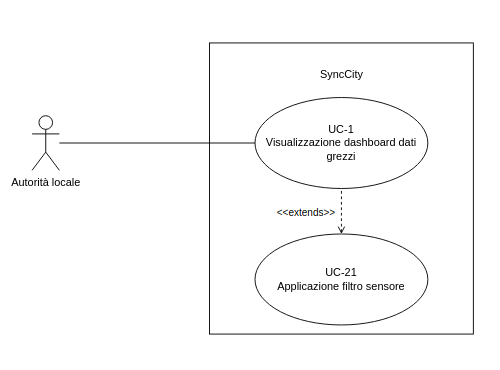
\includegraphics[width=0.6\textwidth]{analisi_dei_requisiti/UC-1.png}
	\captionof{figure}{UC-1: Visualizzazione dashboard dei dati grezzi}
\end{center}

\subsubsubsection{UC-1.1: Visualizzazione \textit{panel} con tabella sensori}
\begin{itemize}
	\item \textbf{Attore principale}: Autorità locale;
	\item \textbf{Precondizioni}:
	      \begin{enumerate}
		      \item L'autorità locale ha effettuato l'accesso al sistema ed esso è in funzione;
	      \end{enumerate}
	\item \textbf{Postcondizioni}:
	      L'autorità locale visualizza il \textit{panel} contenente una tabella di tutti i sensori collegati al sistema;

	\item \textbf{Scenario principale}:
	      \begin{enumerate}
		      \item L'autorità locale accede alla piattaforma;
		      \item Il sistema carica i dati relativi ai sensori interrogando il database;
		      \item L'autorità locale seleziona la visualizzazione della dashboard dei dati grezzi.
	      \end{enumerate}
	\item \href{https://7last.github.io/docs/rtb/documentazione-interna/glossario\#user-story}{\textbf{User story}\textsubscript{G}}: Come autorità locale desidero poter visualizzare un \textit{panel} contenente una tabella di tutti i sensori collegati al sistema.
	      I dati che dovranno essere presenti nella tabella sono: identificativo del sensore, tipo di sensore,
	      e data dell'ultima trasmissione. I dati presenti nella tabella mi consentiranno di avere una visione d'insieme dei sensori presenti.

\end{itemize}
\begin{center}
	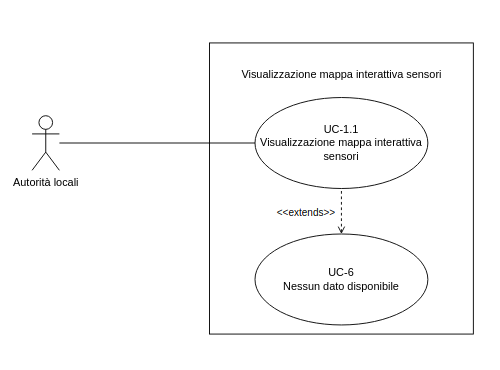
\includegraphics[width=0.6\textwidth]{analisi_dei_requisiti/UC-1.1.png}
	\captionof{figure}{UC-1.1: Visualizzazione \textit{panel} con tabella sensori}
\end{center}

\subsubsubsection{UC-1.2: Visualizzazione mappa interattiva sensori}
\begin{itemize}
	\item \textbf{Attore principale}: Autorità locale;
	\item \textbf{Precondizioni}: L'autorità locale ha effettuato l'accesso al sistema ed esso è in funzione;
	\item \textbf{Postcondizioni}: L'autorità locale visualizza un \textit{panel} contenente una mappa interattiva
	      popolata con dei marker rappresentanti la posizione dei sensori;
	\item \textbf{Scenario principale}:
	      \begin{enumerate}
		      \item L'autorità locale accede alla piattaforma;
		      \item Il sistema carica i dati trasmessi dai sensori interrogando il database;
		      \item L'autorità locale seleziona la visualizzazione della dashboard dei dati grezzi.
	      \end{enumerate}
	\item \href{https://7last.github.io/docs/rtb/documentazione-interna/glossario\#user-story}{\textbf{User story}\textsubscript{G}}: Come autorità locale desidero poter visualizzare una mappa interattiva popolata con dei marker rappresentanti
	      la posizione dei sensori e contenenti il loro identificativo. Essa mi consentirà di visualizzare la distribuzione dei sensori nel territorio
	      ed eventualmente di intervenire nel caso in cui siano presenti zone non coperte.
\end{itemize}
\begin{center}
	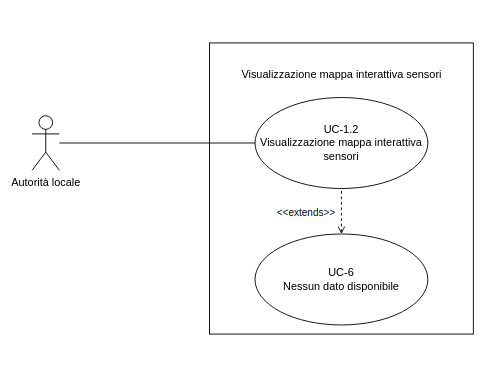
\includegraphics[width=0.6\textwidth]{analisi_dei_requisiti/UC-1.2.png}
	\captionof{figure}{UC-1.2: Visualizzazione mappa interattiva sensori}
\end{center}

\subsubsubsection{UC-1.3: Visualizzazione \textit{panel} numero sensori per tipo}
\begin{itemize}
	\item \textbf{Attore principale}: Autorità locale;
	\item \textbf{Precondizioni}: L'autorità locale ha effettuato l'accesso al sistema ed esso è in funzione;
	\item \textbf{Postcondizioni}: L'autorità locale visualizza un \textit{panel} contenente il conteggio totale di sensori presenti nel sistema;
	\item \textbf{Scenario principale}:
	      \begin{enumerate}
		      \item L'autorità locale accede alla piattaforma;
		      \item Il sistema carica i dati trasmessi dai sensori interrogando il database;
		      \item L'autorità locale seleziona la visualizzazione della dashboard dei dati grezzi.
	      \end{enumerate}
	\item \href{https://7last.github.io/docs/rtb/documentazione-interna/glossario\#user-story}{\textbf{User story}\textsubscript{G}}:
	      Come autorità locale desidero poter visualizzare il conteggio totale di sensori presenti nel sistema suddivisi per tipo, in modo da poter decidere eventualmente di aggiungerne altri.
\end{itemize}
\begin{center}
	
\includegraphics[width=0.6\textwidth]{analisi_dei_requisiti/UC-1.3.png}
	\captionof{figure}{UC-1.3: Visualizzazione \textit{panel} numero sensori per tipo}
\end{center}

\subsubsubsection{UC-1.4: Visualizzazione tabella sensori non trasmettenti}
\begin{itemize}
	\item \textbf{Attore principale}: Autorità locale;
	\item \textbf{Precondizioni}: L'autorità locale ha effettuato l'accesso al sistema ed esso è in funzione;
	\item \textbf{Postcondizioni}: L'autorità locale visualizza una tabella contenente i sensori che non trasmettono da più di un giorno;
	\item \textbf{Scenario principale}:
	      \begin{enumerate}
		      \item L'autorità locale accede alla piattaforma;
		      \item Il sistema carica i dati trasmessi dai sensori interrogando il database;
		      \item L'autorità locale seleziona la visualizzazione della dashboard dei dati grezzi.
	      \end{enumerate}
	\item \href{https://7last.github.io/docs/rtb/documentazione-interna/glossario\#user-story}{\textbf{User story}\textsubscript{G}}:
	      Come autorità locale desidero poter visualizzare una tabella contenente i sensori che non trasmettono da più di un giorno, in modo da poter intervenire e ripristinare il corretto funzionamento.
\end{itemize}
\begin{center}
	
\includegraphics[width=0.6\textwidth]{analisi_dei_requisiti/UC-1.4.png}
	\captionof{figure}{UC-1.4: Visualizzazione tabella sensori che non trasmettono da più di 1 giorno}
\end{center}

\subsubsubsection{UC-1.5: Visualizzazione tabella dati grezzi per tipo di sensore}
\begin{itemize}
	\item \textbf{Attore principale}: Autorità locale;
	\item \textbf{Precondizioni}: L'autorità locale ha effettuato l'accesso al sistema ed esso è in funzione;
	\item \textbf{Postcondizioni}: L'autorità locale visualizza una tabella contenente i dati grezzi trasmessi dai sensori suddivisi per tipo;
	\item \textbf{Scenario principale}:
	      \begin{enumerate}
		      \item L'autorità locale accede alla piattaforma;
		      \item Il sistema carica i dati trasmessi dai sensori interrogando il database;
		      \item L'autorità locale seleziona la visualizzazione della dashboard dei dati grezzi.
	      \end{enumerate}
	\item \href{https://7last.github.io/docs/rtb/documentazione-interna/glossario\#user-story}{\textbf{User story}\textsubscript{G}}:
	      Come autorità locale desidero poter visualizzare una tabella contenente i dati grezzi trasmessi dai sensori suddivisi per tipo, in modo da poter analizzare i dati in modo più dettagliato.
\end{itemize}
\begin{center}
	
\includegraphics[width=0.6\textwidth]{analisi_dei_requisiti/UC-1.5.png}
	\captionof{figure}{UC-1.5: Visualizzazione tabella dati grezzi per tipo di sensore}
\end{center}

\subsubsubsection{UC-1.6: Visualizzazione grafico time series dati grezzi per tipo di sensore}
\begin{itemize}
	\item \textbf{Attore principale}: Autorità locale;
	\item \textbf{Precondizioni}: L'autorità locale ha effettuato l'accesso al sistema ed esso è in funzione;
	\item \textbf{Postcondizioni}: L'autorità locale visualizza un grafico time series contenente i dati grezzi trasmessi dai sensori suddivisi per tipo;
	\item \textbf{Scenario principale}:
	      \begin{enumerate}
		      \item L'autorità locale accede alla piattaforma;
		      \item Il sistema carica i dati trasmessi dai sensori interrogando il database;
		      \item L'autorità locale seleziona la visualizzazione della dashboard dei dati grezzi.
	      \end{enumerate}
	\item \href{https://7last.github.io/docs/rtb/documentazione-interna/glossario\#user-story}{\textbf{User story}\textsubscript{G}}:
	      Come autorità locale desidero poter visualizzare un grafico time series contenente i dati grezzi trasmessi dai sensori suddivisi per tipo, in modo da poter analizzare i dati in modo più dettagliato.
\end{itemize}
\begin{center}
	
\includegraphics[width=0.6\textwidth]{analisi_dei_requisiti/UC-1.6.png}
	\captionof{figure}{UC-1.6: Visualizzazione grafico time series dati grezzi per tipo di sensore}
\end{center}

\subsubsection{UC-2: Visualizzazione dashboard temperatura}
\begin{itemize}
	\item \textbf{Attore principale}: Autorità locale;
	\item \textbf{Precondizioni}: L'autorità locale ha effettuato l'accesso al sistema ed esso è in funzione;
	\item \textbf{Postcondizioni}: L'autorità locale visualizza la dashboard relativa
	      ai sensori di temperatura presenti nella città;
	\item \textbf{Scenario principale}:
	      \begin{enumerate}
		      \item L'autorità locale accede alla piattaforma;
		      \item Il sistema carica i dati trasmessi dai sensori interrogando il database;
		      \item L'autorità locale seleziona la visualizzazione della dashboard relativa ai sensori di temperatura.
	      \end{enumerate}
	\item \href{https://7last.github.io/docs/rtb/documentazione-interna/glossario\#user-story}{\textbf{User story}\textsubscript{G}}:
	      Come autorità locale desidero poter visualizzare una dashboard relativa ai sensori di temperatura presenti nella città, la quale
	      dovrà contenere informazioni utili per monitorare l'andamento della temperatura sulla base di dati storici e in tempo reale, mostrando
	      anche statistiche come la temperatura media, massima e minima nel periodo di tempo selezionato.
\end{itemize}
\begin{center}
	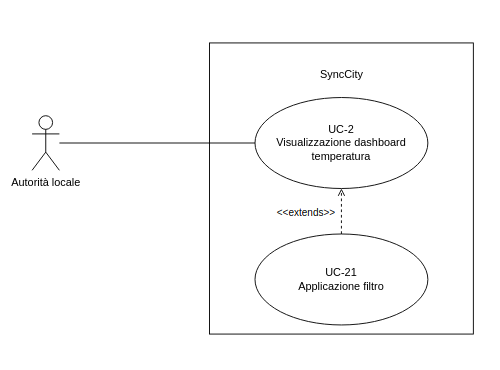
\includegraphics[width=0.6\textwidth]{analisi_dei_requisiti/UC-2.png}
	\captionof{figure}{UC-2: Visualizzazione dashboard temperatura}
\end{center}

\subsubsubsection{UC-2.1: Visualizzazione grafico time series temperatura}
\begin{itemize}
	\item \textbf{Attore principale}: Autorità locale;
	\item \textbf{Precondizioni}:
	      \begin{enumerate}
		      \item L'autorità locale ha effettuato l'accesso al sistema ed esso è in funzione;
		      \item Il sistema ha caricato la dashboard relativa ai sensori di temperatura;
	      \end{enumerate}
	\item \textbf{Postcondizioni}: L'autorità locale visualizza un grafico time series contenente le misurazioni storiche
	      della temperatura aggregate per 5 minuti;
	\item \textbf{Scenario principale}:
	      \begin{enumerate}
		      \item L'autorità locale accede alla piattaforma;
		      \item Il sistema carica i dati relativi ai sensori interrogando il database;
		      \item L'autorità locale seleziona la visualizzazione della dashboard relativa ai sensori di temperatura.
	      \end{enumerate}
	\item \href{https://7last.github.io/docs/rtb/documentazione-interna/glossario\#user-story}{\textbf{User story}\textsubscript{G}}: Come autorità locale desidero poter visualizzare un grafico time series contenente le misurazioni storiche della temperatura
	      per poter monitorarne l'andamento nel tempo e facilmente individuare eventuali anomalie.
\end{itemize}
\begin{center}
	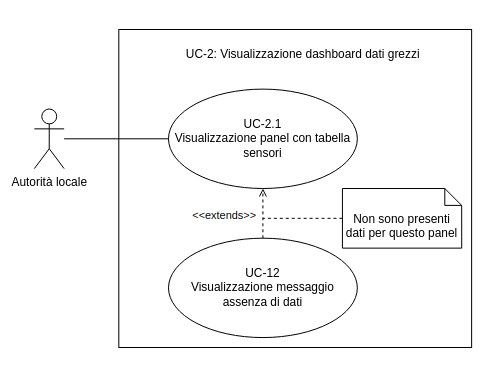
\includegraphics[width=0.75\textwidth]{analisi_dei_requisiti/UC-2.1.png}
	\captionof{figure}{UC-2.1: Visualizzazione grafico time series per temperatura}
\end{center}

\subsubsubsection{UC-2.2: Visualizzazione mappa sensori temperatura}
\begin{itemize}
	\item \textbf{Attore principale}: Autorità locale;
	\item \textbf{Precondizioni}:
	      \begin{enumerate}
		      \item L'autorità locale ha effettuato l'accesso al sistema ed esso è in funzione;
		      \item Il sistema ha caricato la dashboard relativa ai sensori di temperatura;
	      \end{enumerate}
	\item \textbf{Postcondizioni}: L'autorità locale visualizza una mappa interattiva popolata con dei marker rappresentanti la posizione dei sensori di temperatura;
	\item \textbf{Scenario principale}:
	      \begin{enumerate}
		      \item L'autorità locale accede alla piattaforma;
		      \item Il sistema carica i dati relativi ai sensori interrogando il database;
		      \item L'autorità locale seleziona la visualizzazione della dashboard relativa ai sensori di temperatura.
	      \end{enumerate}
	\item \href{https://7last.github.io/docs/rtb/documentazione-interna/glossario\#user-story}{\textbf{User story}\textsubscript{G}}:
	      Come autorità locale desidero poter visualizzare una mappa interattiva popolata con dei marker rappresentanti la posizione dei sensori di temperatura e contenenti il loro identificativo. Essa mi consentirà di visualizzare la distribuzione dei sensori di temperatura nel territorio ed eventualmente interventire nel caso in cui siano presenti zone non coperte.
\end{itemize}
\begin{center}
	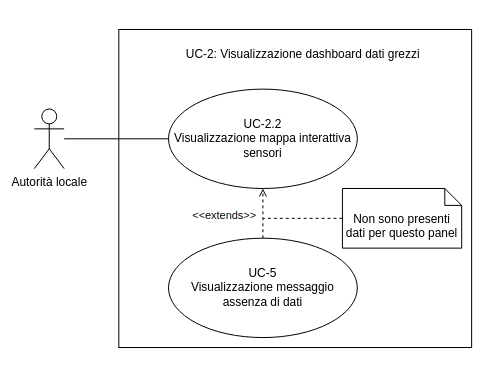
\includegraphics[width=0.75\textwidth]{analisi_dei_requisiti/UC-2.2.png}
	\captionof{figure}{UC-2.2: Visualizzazione mappa interattiva sensori temperatura}
\end{center}

\subsubsubsection{UC-2.3: Visualizzazione \textit{panel} temperatura media nel periodo di tempo selezionato}
\begin{itemize}
	\item \textbf{Attore principale}: Autorità locale;
	\item \textbf{Precondizioni}:
	      \begin{enumerate}
		      \item L'autorità locale ha effettuato l'accesso al sistema ed esso è in funzione;
		      \item Il sistema ha caricato la dashboard relativa ai sensori di temperatura;
	      \end{enumerate}
	\item \textbf{Postcondizioni}: L'autorità locale visualizza un \textit{panel} contenente la temperatura media nel periodo di tempo selezionato;
	\item \textbf{Scenario principale}:
	      \begin{enumerate}
		      \item L'autorità locale accede alla piattaforma;
		      \item Il sistema carica i dati relativi ai sensori interrogando il database;
		      \item L'autorità locale seleziona la visualizzazione della dashboard relativa ai sensori di temperatura.
	      \end{enumerate}
	\item \href{https://7last.github.io/docs/rtb/documentazione-interna/glossario\#user-story}{\textbf{User story}\textsubscript{G}}: Come autorità locale desidero poter visualizzare la temperatura media nel periodo di tempo selezionato
	      in modo da poterne monitorare l'andamento.
\end{itemize}
\begin{center}
	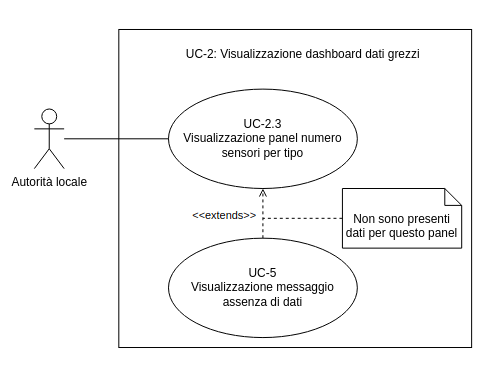
\includegraphics[width=0.75\textwidth]{analisi_dei_requisiti/UC-2.3.png}
	\captionof{figure}{UC-2.3: Visualizzazione \textit{panel} temperatura media nel periodo di tempo selezionato}
\end{center}

\subsubsubsection{UC-2.4: Visualizzazione \textit{panel} temperatura in tempo reale}
\begin{itemize}
	\item \textbf{Attore principale}: Autorità locale;
	\item \textbf{Precondizioni}:
	      \begin{enumerate}
		      \item L'autorità locale ha effettuato l'accesso al sistema ed esso è in funzione;
		      \item Il sistema ha caricato la dashboard relativa ai sensori di temperatura;
	      \end{enumerate}
	\item \textbf{Postcondizioni}: L'autorità locale visualizza un \textit{panel} contenente la temperatura in tempo reale;
	\item \textbf{Scenario principale}:
	      \begin{enumerate}
		      \item L'autorità locale accede alla piattaforma;
		      \item Il sistema carica i dati relativi ai sensori interrogando il database;
		      \item L'autorità locale seleziona la visualizzazione della dashboard relativa ai sensori di temperatura.
	      \end{enumerate}
	\item \href{https://7last.github.io/docs/rtb/documentazione-interna/glossario\#user-story}{\textbf{User story}\textsubscript{G}}:
	      Come autorità locale desidero poter visualizzare la temperatura in tempo reale in modo da poterne monitorare l'andamento
	      e poterla facilmente confrontare con i dati storici.
\end{itemize}
\begin{center}
	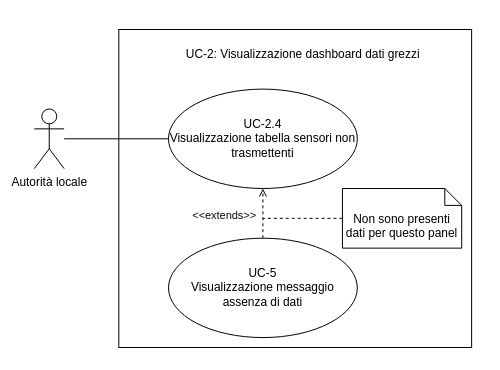
\includegraphics[width=0.75\textwidth]{analisi_dei_requisiti/UC-2.4.png}
	\captionof{figure}{UC-2.4: Visualizzazione \textit{panel} temperatura in tempo reale}
\end{center}

\subsubsubsection{UC-2.5: Visualizzazione \textit{panel} temperatura massima nel periodo di tempo selezionato}
\begin{itemize}
	\item \textbf{Attore principale}: Autorità locale;
	\item \textbf{Precondizioni}:
	      \begin{enumerate}
		      \item L'autorità locale ha effettuato l'accesso al sistema ed esso è in funzione;
		      \item Il sistema ha caricato la dashboard relativa ai sensori di temperatura;
	      \end{enumerate}
	\item \textbf{Postcondizioni}: L'autorità locale visualizza un \textit{panel} contenente la temperatura massima nel periodo di tempo selezionato;
	\item \textbf{Scenario principale}:
	      \begin{enumerate}
		      \item L'autorità locale accede alla piattaforma;
		      \item Il sistema carica i dati relativi ai sensori interrogando il database;
		      \item L'autorità locale seleziona la visualizzazione della dashboard relativa ai sensori di temperatura.
	      \end{enumerate}
	\item \href{https://7last.github.io/docs/rtb/documentazione-interna/glossario\#user-story}{\textbf{User story}\textsubscript{G}}:
	      Come autorità locale desidero poter visualizzare la temperatura massima nel periodo di tempo selezionato
	      in modo da poterla prendere come riferimento e confrontarla con la temperatura attuale.
\end{itemize}
\begin{center}
	
\includegraphics[width=0.75\textwidth]{analisi_dei_requisiti/UC-2.5.png}
	\captionof{figure}{UC-2.5: Visualizzazione \textit{panel} temperatura massima}
\end{center}

\subsubsubsection{UC-2.6: Visualizzazione \textit{panel} temperatura minima nel periodo di tempo selezionato}
\begin{itemize}
	\item \textbf{Attore principale}: Autorità locale;
	\item \textbf{Precondizioni}:
	      \begin{enumerate}
		      \item L'autorità locale ha effettuato l'accesso al sistema ed esso è in funzione;
		      \item Il sistema ha caricato la dashboard relativa ai sensori di temperatura;
	      \end{enumerate}
	\item \textbf{Postcondizioni}: L'autorità locale visualizza un \textit{panel} contenente la temperatura minima nel periodo di tempo selezionato;
	      \begin{enumerate}
		      \item L'autorità locale ha effettuato l'accesso al sistema ed esso è in funzione;
		      \item Il sistema ha caricato la dashboard relativa ai sensori di temperatura;
	      \end{enumerate}
	\item \textbf{Postcondizioni}: L'autorità locale visualizza un \textit{panel} contenente la temperatura minima nel periodo di tempo selezionato;
	\item \textbf{Scenario principale}:
	      \begin{enumerate}
		      \item L'autorità locale accede alla piattaforma;
		      \item Il sistema carica i dati relativi ai sensori interrogando il database;
		      \item L'autorità locale seleziona la visualizzazione della dashboard relativa ai sensori di temperatura.
	      \end{enumerate}
	\item \href{https://7last.github.io/docs/rtb/documentazione-interna/glossario\#user-story}{\textbf{User story}\textsubscript{G}}:
	      Come autorità locale desidero poter visualizzare la temperatura minima nel periodo di tempo selezionato
	      in modo da poterla prendere come riferimento e confrontarla con la temperatura attuale.
\end{itemize}
\begin{center}
	
\includegraphics[width=0.75\textwidth]{analisi_dei_requisiti/UC-2.6.png}
	\captionof{figure}{UC-2.6: Visualizzazione \textit{panel} temperatura minima}
\end{center}

\subsubsection{UC-3: Visualizzazione dashboard umidità}
\begin{itemize}
	\item \textbf{Attore principale}: Autorità locale;
	\item \textbf{Precondizioni}: L'autorità locale ha effettuato l'accesso al sistema ed esso è in funzione;
	\item \textbf{Postcondizioni}: L'autorità locale visualizza la dashboard relativa
	      ai sensori di umidità presenti nella città;
	\item \textbf{Scenario principale}:
	      \begin{enumerate}
		      \item L'autorità locale accede alla piattaforma;
		      \item Il sistema carica i dati trasmessi dai sensori interrogando il database;
		      \item L'autorità locale seleziona la visualizzazione della dashboard relativa ai sensori di umidità.
	      \end{enumerate}
	\item \href{https://7last.github.io/docs/rtb/documentazione-interna/glossario\#user-story}{\textbf{User story}\textsubscript{G}}:
	      Come autorità locale desidero poter visualizzare una dashboard relativa ai sensori di umidità presenti nella città, la quale
	      dovrà contenere informazioni utili per monitorare l'andamento dell'umidità sulla base di dati storici e in tempo reale, mostrando
	      anche statistiche come l'umidità media, massima e minima nel periodo di tempo selezionato.
\end{itemize}
\begin{center}
	
\includegraphics[width=0.6\textwidth]{analisi_dei_requisiti/UC-3.png}
	\captionof{figure}{UC-3: Visualizzazione dashboard umidità}
\end{center}

\subsubsubsection{UC-3.1: Visualizzazione grafico time series umidità}
\begin{itemize}
	\item \textbf{Attore principale}: Autorità locale;
	\item \textbf{Precondizioni}:
	      \begin{enumerate}
		      \item L'autorità locale ha effettuato l'accesso al sistema ed esso è in funzione;
		      \item Il sistema ha caricato la dashboard relativa ai sensori di umidità
	      \end{enumerate}
	\item \textbf{Postcondizioni}: L'autorità locale visualizza un grafico time series contenente le misurazioni storiche
	      di umidità aggregate per 5 minuti;;
	\item \textbf{Scenario principale}:
	      \begin{enumerate}
		      \item L'autorità locale accede alla piattaforma;
		      \item Il sistema carica i dati relativi ai sensori interrogando il database;
		      \item L'autorità locale seleziona la visualizzazione della dashboard relativa ai sensori di umidità;
	      \end{enumerate}
	\item \href{https://7last.github.io/docs/rtb/documentazione-interna/glossario\#user-story}{\textbf{User story}\textsubscript{G}}:
	      Come autorità locale desidero poter visualizzare un grafico time series contenente le misurazioni storiche
	      di umidità per poter monitorarne l'andamento nel tempo e facilmente individuare eventuali anomalie.
\end{itemize}
\begin{center}
	
\includegraphics[width=0.75\textwidth]{analisi_dei_requisiti/UC-3.1.png}
	\captionof{figure}{UC-3.1, Visualizzazione grafico time series umidità}
\end{center}

\subsubsubsection{UC-3.2: Visualizzazione mappa sensori umidità}
\begin{itemize}
	\item \textbf{Attore principale}: Autorità locale;
	\item \textbf{Precondizioni}:
	      \begin{enumerate}
		      \item L'autorità locale ha effettuato l'accesso al sistema ed esso è in funzione;
		      \item Il sistema ha caricato la dashboard relativa ai sensori di umidità;
	      \end{enumerate}
	\item \textbf{Postcondizioni}: L'autorità locale visualizza una mappa interattiva popolata con dei marker rappresentanti la posizione dei sensori di umidità;
	\item \textbf{Scenario principale}:
	      \begin{enumerate}
		      \item L'autorità locale accede alla piattaforma;
		      \item Il sistema carica i dati relativi ai sensori interrogando il database;
		      \item L'autorità locale seleziona la visualizzazione della dashboard relativa ai sensori di umidità.
	      \end{enumerate}
	\item \href{https://7last.github.io/docs/rtb/documentazione-interna/glossario\#user-story}{\textbf{User story}\textsubscript{G}}:
	      Come autorità locale desidero poter visualizzare una mappa interattiva popolata con dei marker rappresentanti la posizione dei sensori di umidità
	      e contenenti il loro identificativo. Essa mi consentirà di visualizzare la distribuzione dei sensori di umidità nel territorio ed eventualmente interventire nel caso in cui siano presenti zone non coperte.
\end{itemize}
\begin{center}
	
\includegraphics[width=0.75\textwidth]{analisi_dei_requisiti/UC-3.2.png}
	\captionof{figure}{UC-3.2: Visualizzazione mappa interattiva sensori umidità}
\end{center}

\subsubsubsection{UC-3.3: Visualizzazione \textit{panel} umidità media nel periodo di tempo selezionato}
\begin{itemize}
	\item \textbf{Attore principale}: Autorità locale;
	\item \textbf{Precondizioni}:
	      \begin{enumerate}
		      \item L'autorità locale ha effettuato l'accesso al sistema ed esso è in funzione;
		      \item Il sistema ha caricato la dashboard relativa ai sensori di umidità;
	      \end{enumerate}
	\item \textbf{Postcondizioni}: L'autorità locale visualizza un \textit{panel} contenente l'umidità media nel periodo di tempo selezionato;
	\item \textbf{Scenario principale}:
	      \begin{enumerate}
		      \item L'autorità locale accede alla piattaforma;
		      \item Il sistema carica i dati relativi ai sensori interrogando il database;
		      \item L'autorità locale seleziona la visualizzazione della dashboard relativa ai sensori di umidità.
	      \end{enumerate}
	\item \href{https://7last.github.io/docs/rtb/documentazione-interna/glossario\#user-story}{\textbf{User story}\textsubscript{G}}: Come autorità locale desidero poter visualizzare l'umidità media nel periodo di tempo selezionato
	      in modo da poterne monitorare l'andamento.
\end{itemize}
\begin{center}
	
\includegraphics[width=0.75\textwidth]{analisi_dei_requisiti/UC-3.3.png}
	\captionof{figure}{UC-3.3: Visualizzazione \textit{panel} umidità media nel periodo di tempo selezionato}
\end{center}

\subsubsubsection{UC-3.4: Visualizzazione \textit{panel} umidità in tempo reale}
\begin{itemize}
	\item \textbf{Attore principale}: Autorità locale;
	\item \textbf{Precondizioni}:
	      \begin{enumerate}
		      \item L'autorità locale ha effettuato l'accesso al sistema ed esso è in funzione;
		      \item Il sistema ha caricato la dashboard relativa ai sensori di umidità;
	      \end{enumerate}
	\item \textbf{Postcondizioni}: L'autorità locale visualizza un \textit{panel} contenente l'umidità in tempo reale;
	\item \textbf{Scenario principale}:
	      \begin{enumerate}
		      \item L'autorità locale accede alla piattaforma;
		      \item Il sistema carica i dati relativi ai sensori interrogando il database;
		      \item L'autorità locale seleziona la visualizzazione della dashboard relativa ai sensori di umidità.
	      \end{enumerate}
	\item \href{https://7last.github.io/docs/rtb/documentazione-interna/glossario\#user-story}{\textbf{User story}\textsubscript{G}}:
	      Come autorità locale desidero poter visualizzare l'umidità in tempo reale in modo da poterne monitorare l'andamento
	      e poterla facilmente confrontare con i dati storici.
\end{itemize}
\begin{center}
	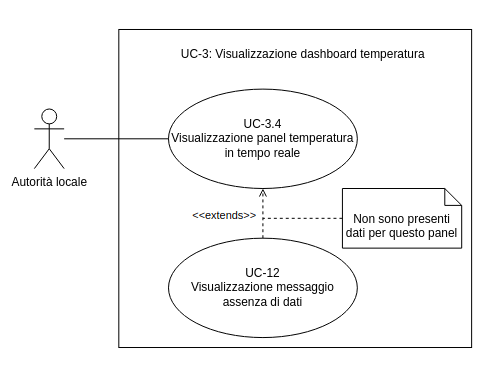
\includegraphics[width=0.75\textwidth]{analisi_dei_requisiti/UC-3.4.png}
	\captionof{figure}{UC-3.4: Visualizzazione \textit{panel} umidità in tempo reale}
\end{center}

\subsubsubsection{UC-3.5: Visualizzazione \textit{panel} umidità massima nel periodo di tempo selezionato}
\begin{itemize}
	\item \textbf{Attore principale}: Autorità locale;
	\item \textbf{Precondizioni}:
	      \begin{enumerate}
		      \item L'autorità locale ha effettuato l'accesso al sistema ed esso è in funzione;
		      \item Il sistema ha caricato la dashboard relativa ai sensori di umidità;
	      \end{enumerate}
	\item \textbf{Postcondizioni}: L'autorità locale visualizza un \textit{panel} contenente l'umidità massima nel periodo di tempo selezionato;
	\item \textbf{Scenario principale}:
	      \begin{enumerate}
		      \item L'autorità locale accede alla piattaforma;
		      \item Il sistema carica i dati relativi ai sensori interrogando il database;
		      \item L'autorità locale seleziona la visualizzazione della dashboard relativa ai sensori di umidità.
	      \end{enumerate}
	\item \href{https://7last.github.io/docs/rtb/documentazione-interna/glossario\#user-story}{\textbf{User story}\textsubscript{G}}:
	      Come autorità locale desidero poter visualizzare l'umidità massima nel periodo di tempo selezionato
	      in modo da poterla prendere come riferimento e confrontarla con l'umidità attuale.
\end{itemize}
\begin{center}
	
\includegraphics[width=0.75\textwidth]{analisi_dei_requisiti/UC-3.5.png}
	\captionof{figure}{UC-3.5: Visualizzazione \textit{panel} umidità massima}
\end{center}

\subsubsubsection{UC-3.6: Visualizzazione \textit{panel} umidità minima nel periodo di tempo selezionato}
\begin{itemize}
	\item \textbf{Attore principale}: Autorità locale;
	\item \textbf{Precondizioni}:
	      \begin{enumerate}
		      \item L'autorità locale ha effettuato l'accesso al sistema ed esso è in funzione;
		      \item Il sistema ha caricato la dashboard relativa ai sensori di umidità;
	      \end{enumerate}
	\item \textbf{Postcondizioni}: L'autorità locale visualizza un \textit{panel} contenente l'umidità minima nel periodo di tempo selezionato;
	\item \textbf{Scenario principale}:
	      \begin{enumerate}
		      \item L'autorità locale accede alla piattaforma;
		      \item Il sistema carica i dati relativi ai sensori interrogando il database;
		      \item L'autorità locale seleziona la visualizzazione della dashboard relativa ai sensori di umidità.
	      \end{enumerate}
	\item \href{https://7last.github.io/docs/rtb/documentazione-interna/glossario\#user-story}{\textbf{User story}\textsubscript{G}}:
	      Come autorità locale desidero poter visualizzare l'umidità minima nel periodo di tempo selezionato
	      in modo da poterla prendere come riferimento e confrontarla con l'umidità attuale.
\end{itemize}
\begin{center}
	
\includegraphics[width=0.75\textwidth]{analisi_dei_requisiti/UC-3.6.png}
	\captionof{figure}{UC-3.6: Visualizzazione \textit{panel} umidità minima}
\end{center}

\subsubsection{UC-4: Visualizzazione dashboard qualità dell'aria}
\begin{itemize}
	\item \textbf{Attore principale}: Autorità locale;
	\item \textbf{Precondizioni}: L'autorità locale ha effettuato l'accesso al sistema ed esso è in funzione;
	\item \textbf{Postcondizioni}: L'autorità locale visualizza la dashboard relativa
	      ai sensori di qualità dell'aria presenti nella città;
	\item \textbf{Scenario principale}:
	      \begin{enumerate}
		      \item L'autorità locale accede alla piattaforma;
		      \item Il sistema carica i dati trasmessi dai sensori interrogando il database;
		      \item L'autorità locale seleziona la visualizzazione della dashboard relativa ai sensori di qualità dell'aria.
	      \end{enumerate}
	\item \href{https://7last.github.io/docs/rtb/documentazione-interna/glossario\#user-story}{\textbf{User story}\textsubscript{G}}:
	      Come autorità locale desidero poter visualizzare una dashboard relativa ai sensori di qualità dell'aria presenti nella città, la quale
	      dovrà contenere informazioni utili per monitorare l'andamento della qualità dell'aria sulla base di dati storici e in tempo reale, mostrando
	      anche statistiche quali il giorno con la qualità dell'aria peggiore e il giorno con la qualità dell'aria migliore nel periodo di tempo selezionato.
\end{itemize}
\begin{center}
	
\includegraphics[width=0.6\textwidth]{analisi_dei_requisiti/UC-4.png}
	\captionof{figure}{UC-4: Visualizzazione dashboard qualità dell'aria}
\end{center}

\subsubsubsection{UC-4.1: Visualizzazione grafico time series qualità dell'aria}
\begin{itemize}
	\item \textbf{Attore principale}: Autorità locale;
	\item \textbf{Precondizioni}:
	      \begin{enumerate}
		      \item L'autorità locale ha effettuato l'accesso al sistema ed esso è in funzione;
		      \item Il sistema ha caricato la dashboard relativa ai sensori di qualità dell'aria
	      \end{enumerate}
	\item \textbf{Postcondizioni}: L'autorità locale visualizza un grafico time series contenente le misurazioni storiche
	      di qualità dell'aria aggregate per 5 minuti;
	\item \textbf{Scenario principale}:
	      \begin{enumerate}
		      \item L'autorità locale accede alla piattaforma;
		      \item Il sistema carica i dati relativi ai sensori interrogando il database;
		      \item L'autorità locale seleziona la visualizzazione della dashboard relativa ai sensori di qualità dell'aria;
	      \end{enumerate}
	\item \href{https://7last.github.io/docs/rtb/documentazione-interna/glossario\#user-story}{\textbf{User story}\textsubscript{G}}:
	      Come autorità locale desidero poter visualizzare un grafico time series contenente le misurazioni storiche
	      di qualità dell'aria per poter monitorarne l'andamento nel tempo e facilmente individuare eventuali anomalie.
\end{itemize}
\begin{center}
	
\includegraphics[width=0.75\textwidth]{analisi_dei_requisiti/UC-4.1.png}
	\captionof{figure}{UC-4.1, Visualizzazione grafico time series qualità dell'aria}
\end{center}

\subsubsubsection{UC-4.2: Visualizzazione mappa interattiva sensori qualità dell'aria}
\begin{itemize}
	\item \textbf{Attore principale}: Autorità locale;
	\item \textbf{Precondizioni}:
	      \begin{enumerate}
		      \item L'autorità locale ha effettuato l'accesso al sistema ed esso è in funzione;
		      \item Il sistema ha caricato la dashboard relativa ai sensori di qualità dell'aria;
	      \end{enumerate}
	\item \textbf{Postcondizioni}: L'autorità locale visualizza una mappa interattiva popolata con dei marker rappresentanti la posizione dei sensori della qualità dell'aria;
	\item \textbf{Scenario principale}:
	      \begin{enumerate}
		      \item L'autorità locale accede alla piattaforma;
		      \item Il sistema carica i dati relativi ai sensori interrogando il database;
		      \item L'autorità locale seleziona la visualizzazione della dashboard relativa ai sensori della qualità dell'aria.
	      \end{enumerate}
	\item \href{https://7last.github.io/docs/rtb/documentazione-interna/glossario\#user-story}{\textbf{User story}\textsubscript{G}}:
	      Come autorità locale desidero poter visualizzare una mappa interattiva popolata con dei marker rappresentanti la posizione dei sensori della qualità dell'aria
	      e contenenti il loro identificativo. Essa mi consentirà di visualizzare la distribuzione dei sensori della qualità dell'aria nel territorio ed eventualmente interventire nel caso in cui siano presenti zone non coperte.
\end{itemize}
\begin{center}
	
\includegraphics[width=0.75\textwidth]{analisi_dei_requisiti/UC-4.2.png}
	\captionof{figure}{UC-4.2: Visualizzazione mappa interattiva sensori qualità dell'aria}
\end{center}

\subsubsubsection{UC-4.3: Visualizzazione \textit{panel} qualità dell'aria media nel periodo di tempo selezionato}
\begin{itemize}
	\item \textbf{Attore principale}: Autorità locale;
	\item \textbf{Precondizioni}:
	      \begin{enumerate}
		      \item L'autorità locale ha effettuato l'accesso al sistema ed esso è in funzione;
		      \item Il sistema ha caricato la dashboard relativa ai sensori di qualità dell'aria;
	      \end{enumerate}
	\item \textbf{Postcondizioni}: L'autorità locale visualizza un \textit{panel} contenente qualità dell'aria media nel periodo di tempo selezionato;
	\item \textbf{Scenario principale}:
	      \begin{enumerate}
		      \item L'autorità locale accede alla piattaforma;
		      \item Il sistema carica i dati relativi ai sensori interrogando il database;
		      \item L'autorità locale seleziona la visualizzazione della dashboard relativa ai sensori di qualità dell'aria.
	      \end{enumerate}
	\item \href{https://7last.github.io/docs/rtb/documentazione-interna/glossario\#user-story}{\textbf{User story}\textsubscript{G}}: Come autorità locale desidero poter visualizzare della qualità dell'aria media nel periodo di tempo selezionato
	      in modo da poterne monitorare l'andamento.
\end{itemize}
\begin{center}
	
\includegraphics[width=0.75\textwidth]{analisi_dei_requisiti/UC-4.3.png}
	\captionof{figure}{UC-4.3: Visualizzazione \textit{panel} qualità dell'aria media nel periodo di tempo selezionato}
\end{center}

\subsubsubsection{UC-4.4: Visualizzazione \textit{panel} qualità dell'aria in tempo reale}
\begin{itemize}
	\item \textbf{Attore principale}: Autorità locale;
	\item \textbf{Precondizioni}:
	      \begin{enumerate}
		      \item L'autorità locale ha effettuato l'accesso al sistema ed esso è in funzione;
		      \item Il sistema ha caricato la dashboard relativa ai sensori di qualità dell'aria;
	      \end{enumerate}
	\item \textbf{Postcondizioni}: L'autorità locale visualizza un \textit{panel} contenente qualità dell'aria in tempo reale;
	\item \textbf{Scenario principale}:
	      \begin{enumerate}
		      \item L'autorità locale accede alla piattaforma;
		      \item Il sistema carica i dati relativi ai sensori interrogando il database;
		      \item L'autorità locale seleziona la visualizzazione della dashboard relativa ai sensori di qualità dell'aria.
	      \end{enumerate}
	\item \href{https://7last.github.io/docs/rtb/documentazione-interna/glossario\#user-story}{\textbf{User story}\textsubscript{G}}:
	      Come autorità locale desidero poter visualizzare della qualità dell'aria in tempo reale in modo da poterne monitorare l'andamento
	      e poterla facilmente confrontare con i dati storici.
\end{itemize}
\begin{center}
	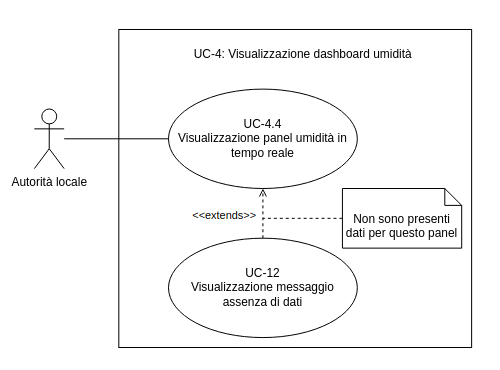
\includegraphics[width=0.75\textwidth]{analisi_dei_requisiti/UC-4.4.png}
	\captionof{figure}{UC-4.4: Visualizzazione \textit{panel} qualità dell'aria in tempo reale}
\end{center}
\subsubsubsection{UC-4.5: Visualizzazione \textit{panel} giorno con qualità dell'aria peggiore nel periodo di tempo selezionato}
\begin{itemize}
	\item \textbf{Attore principale}: Autorità locale;
	\item \textbf{Precondizioni}:
	      \begin{enumerate}
		      \item L'autorità locale ha effettuato l'accesso al sistema ed esso è in funzione;
		      \item Il sistema ha caricato la dashboard relativa ai sensori di qualità dell'aria;
	      \end{enumerate}
	\item \textbf{Postcondizioni}: L'autorità locale visualizza un \textit{panel} contenente il giorno con la qualità dell'aria peggiore nel periodo di tempo selezionato;
	\item \textbf{Scenario principale}:
	      \begin{enumerate}
		      \item L'autorità locale accede alla piattaforma;
		      \item Il sistema carica i dati relativi ai sensori interrogando il database;
		      \item L'autorità locale seleziona la visualizzazione della dashboard relativa ai sensori di qualità dell'aria.
	      \end{enumerate}
	\item \href{https://7last.github.io/docs/rtb/documentazione-interna/glossario\#user-story}{\textbf{User story}\textsubscript{G}}:
	      Come autorità locale desidero poter visualizzare il giorno con la qualità dell'aria peggiore nel periodo di tempo selezionato
	      in modo da poterla prendere come riferimento e confrontarla con la qualità dell'aria attuale.
\end{itemize}
\begin{center}
	
\includegraphics[width=0.75\textwidth]{analisi_dei_requisiti/UC-4.5.png}
	\captionof{figure}{UC-4.5: Visualizzazione \textit{panel} giorno con qualità dell'aria peggiore nel periodo di tempo selezionato}
\end{center}

\subsubsubsection{UC-4.6: Visualizzazione \textit{panel} giorno con qualità dell'aria migliore nel periodo di tempo selezionato}
\begin{itemize}
	\item \textbf{Attore principale}: Autorità locale;
	\item \textbf{Precondizioni}:
	      \begin{enumerate}
		      \item L'autorità locale ha effettuato l'accesso al sistema ed esso è in funzione;
		      \item Il sistema ha caricato la dashboard relativa ai sensori di qualità dell'aria;
	      \end{enumerate}
	\item \textbf{Postcondizioni}: L'autorità locale visualizza un \textit{panel} contenente il giorno con la qualità dell'aria migliore nel periodo di tempo selezionato;
	\item \textbf{Scenario principale}:
	      \begin{enumerate}
		      \item L'autorità locale accede alla piattaforma;
		      \item Il sistema carica i dati relativi ai sensori interrogando il database;
		      \item L'autorità locale seleziona la visualizzazione della dashboard relativa ai sensori di qualità dell'aria.
	      \end{enumerate}
	\item \href{https://7last.github.io/docs/rtb/documentazione-interna/glossario\#user-story}{\textbf{User story}\textsubscript{G}}:
	      Come autorità locale desidero poter visualizzare il giorno con la qualità dell'aria migliore nel periodo di tempo selezionato
	      in modo da poterla prendere come riferimento e confrontarla con la qualità dell'aria attuale.
\end{itemize}
\begin{center}
	
\includegraphics[width=0.75\textwidth]{analisi_dei_requisiti/UC-4.6.png}
	\captionof{figure}{UC-4.6: Visualizzazione \textit{panel} giorno con qualità dell'aria peggiore nel periodo di tempo selezionato}
\end{center}

\subsubsection{UC-5: Visualizzazione dashboard precipitazioni}
\begin{itemize}
	\item \textbf{Attore principale}: Autorità locale;
	\item \textbf{Precondizioni}: L'autorità locale ha effettuato l'accesso al sistema ed esso è in funzione;
	\item \textbf{Postcondizioni}: L'autorità locale visualizza la dashboard relativa
	      ai sensori di precipitazioni presenti nella città;
	\item \textbf{Scenario principale}:
	      \begin{enumerate}
		      \item L'autorità locale accede alla piattaforma;
		      \item Il sistema carica i dati trasmessi dai sensori interrogando il database;
		      \item L'autorità locale seleziona la visualizzazione della dashboard relativa ai sensori di precipitazioni.
	      \end{enumerate}
	\item \href{https://7last.github.io/docs/rtb/documentazione-interna/glossario\#user-story}{\textbf{User story}\textsubscript{G}}:
	      Come autorità locale desidero poter visualizzare una dashboard relativa ai sensori di precipitazioni presenti nella città, la quale
	      dovrà contenere informazioni utili per monitorare l'andamento dele precipitazioni sulla base di dati storici e in tempo reale, mostrando
	      anche statistiche quali quantità di precipitazioni media, massima e minima nel periodo di tempo selezionato.
\end{itemize}
\begin{center}
	
\includegraphics[width=0.6\textwidth]{analisi_dei_requisiti/UC-5.png}
	\captionof{figure}{UC-5: Visualizzazione dashboard precipitazioni}
\end{center}

\subsubsubsection{UC-5.1: Visualizzazione grafico time series quantità precipitazioni nel periodo di tempo selezionato}
\begin{itemize}
	\item \textbf{Attore principale}: Autorità locale;
	\item \textbf{Precondizioni}:
	      \begin{enumerate}
		      \item L'autorità locale ha effettuato l'accesso al sistema ed esso è in funzione;
		      \item Il sistema ha caricato la dashboard relativa ai sensori di precipitazioni
	      \end{enumerate}
	\item \textbf{Postcondizioni}: L'autorità locale visualizza un grafico time series contenente le misurazioni storiche
	      di precipitazioni aggregate per 5 minuti;
	\item \textbf{Scenario principale}:
	      \begin{enumerate}
		      \item L'autorità locale accede alla piattaforma;
		      \item Il sistema carica i dati relativi ai sensori interrogando il database;
		      \item L'autorità locale seleziona la visualizzazione della dashboard relativa ai sensori di precipitazioni;
	      \end{enumerate}
	\item \href{https://7last.github.io/docs/rtb/documentazione-interna/glossario\#user-story}{\textbf{User story}\textsubscript{G}}:
	      Come autorità locale desidero poter visualizzare un grafico time series contenente le misurazioni storiche
	      di precipitazioni per poter monitorarne l'andamento nel tempo e facilmente individuare eventuali anomalie.
\end{itemize}
\begin{center}
	
\includegraphics[width=0.75\textwidth]{analisi_dei_requisiti/UC-5.1.png}
	\captionof{figure}{UC-5.1, Visualizzazione grafico time series precipitazioni}
\end{center}

\subsubsubsection{UC-5.2: Visualizzazione mappa sensori precipitazioni}
\begin{itemize}
	\item \textbf{Attore principale}: Autorità locale;
	\item \textbf{Precondizioni}:
	      \begin{enumerate}
		      \item L'autorità locale ha effettuato l'accesso al sistema ed esso è in funzione;
		      \item Il sistema ha caricato la dashboard relativa ai sensori di precipitazioni;
	      \end{enumerate}
	\item \textbf{Postcondizioni}: L'autorità locale visualizza una mappa interattiva popolata con dei marker rappresentanti la posizione dei sensori di precipitazioni;
	\item \textbf{Scenario principale}:
	      \begin{enumerate}
		      \item L'autorità locale accede alla piattaforma;
		      \item Il sistema carica i dati relativi ai sensori interrogando il database;
		      \item L'autorità locale seleziona la visualizzazione della dashboard relativa ai sensori di precipitazioni.
	      \end{enumerate}
	\item \href{https://7last.github.io/docs/rtb/documentazione-interna/glossario\#user-story}{\textbf{User story}\textsubscript{G}}:
	      Come autorità locale desidero poter visualizzare una mappa interattiva popolata con dei marker rappresentanti la posizione dei sensori di precipitazioni
	      e contenenti il loro identificativo. Essa mi consentirà di visualizzare la distribuzione dei sensori di precipitazioni nel territorio ed
	      eventualmente interventire nel caso in cui siano presenti zone non coperte.
\end{itemize}
\begin{center}
	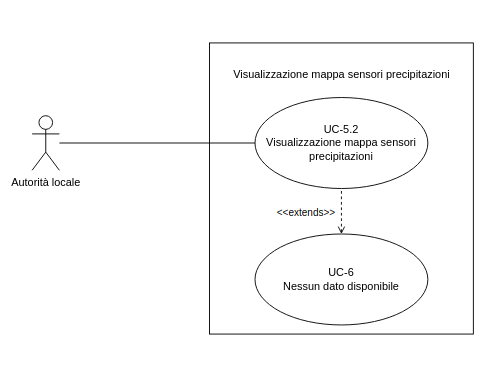
\includegraphics[width=0.75\textwidth]{analisi_dei_requisiti/UC-5.2.png}
	\captionof{figure}{UC-5.2: Visualizzazione mappa interattiva sensori precipitazioni}
\end{center}


\subsubsubsection{UC-5.3: Visualizzazione \textit{panel} quantità di precipitazioni media nel periodo di tempo selezionato}
\begin{itemize}
	\item \textbf{Attore principale}: Autorità locale;
	\item \textbf{Precondizioni}:
	      \begin{enumerate}
		      \item L'autorità locale ha effettuato l'accesso al sistema ed esso è in funzione;
		      \item Il sistema ha caricato la dashboard relativa ai sensori di quantità di precipitazioni;
	      \end{enumerate}
	\item \textbf{Postcondizioni}: L'autorità locale visualizza un \textit{panel} contenente di quantità di precipitazioni media nel periodo di tempo selezionato;
	\item \textbf{Scenario principale}:
	      \begin{enumerate}
		      \item L'autorità locale accede alla piattaforma;
		      \item Il sistema carica i dati relativi ai sensori interrogando il database;
		      \item L'autorità locale seleziona la visualizzazione della dashboard relativa ai sensori di quantità di precipitazioni.
	      \end{enumerate}
	\item \href{https://7last.github.io/docs/rtb/documentazione-interna/glossario\#user-story}{\textbf{User story}\textsubscript{G}}: Come autorità locale desidero poter visualizzare di quantità di precipitazioni media nel periodo di tempo selezionato
	      in modo da poterne monitorare l'andamento.
\end{itemize}
\begin{center}
	
\includegraphics[width=0.75\textwidth]{analisi_dei_requisiti/UC-5.3.png}
	\captionof{figure}{UC-5.3: Visualizzazione \textit{panel} quantità di precipitazioni media nel periodo di tempo selezionato}
\end{center}

\subsubsubsection{UC-5.4: Visualizzazione \textit{panel} quantità di precipitazioni in tempo reale}
\begin{itemize}
	\item \textbf{Attore principale}: Autorità locale;
	\item \textbf{Precondizioni}:
	      \begin{enumerate}
		      \item L'autorità locale ha effettuato l'accesso al sistema ed esso è in funzione;
		      \item Il sistema ha caricato la dashboard relativa ai sensori di quantità di precipitazioni;
	      \end{enumerate}
	\item \textbf{Postcondizioni}: L'autorità locale visualizza un \textit{panel} contenente di quantità di precipitazioni in tempo reale;
	\item \textbf{Scenario principale}:
	      \begin{enumerate}
		      \item L'autorità locale accede alla piattaforma;
		      \item Il sistema carica i dati relativi ai sensori interrogando il database;
		      \item L'autorità locale seleziona la visualizzazione della dashboard relativa ai sensori di quantità di precipitazioni.
	      \end{enumerate}
	\item \href{https://7last.github.io/docs/rtb/documentazione-interna/glossario\#user-story}{\textbf{User story}\textsubscript{G}}:
	      Come autorità locale desidero poter visualizzare di quantità di precipitazioni in tempo reale in modo da poterne monitorare l'andamento
	      e poterla facilmente confrontare con i dati storici.
\end{itemize}
\begin{center}
	
\includegraphics[width=0.75\textwidth]{analisi_dei_requisiti/UC-5.3.png}
	\captionof{figure}{UC-5.3: Visualizzazione \textit{panel} quantità di precipitazioni in tempo reale}
\end{center}

\subsubsubsection{UC-5.5: Visualizzazione \textit{panel} giorno con precipitazioni maggiori nel periodo di tempo selezionato}
\subsubsubsection{UC-5.6: Visualizzazione \textit{panel} giorno con precipitazioni minori nel periodo di tempo selezionato}

\subsubsection{UC-6: Visualizzazione dashboard traffico}
\begin{itemize}
	\item \textbf{Attore principale}: Autorità locale;
	\item \textbf{Precondizioni}: L'autorità locale ha effettuato l'accesso al sistema ed esso è in funzione;
	\item \textbf{Postcondizioni}: L'autorità locale visualizza la dashboard relativa
	      ai sensori di traffico presenti nella città;
	\item \textbf{Scenario principale}:
	      \begin{enumerate}
		      \item L'autorità locale accede alla piattaforma;
		      \item Il sistema carica i dati trasmessi dai sensori interrogando il database;
		      \item L'autorità locale seleziona la visualizzazione della dashboard relativa ai sensori di traffico.
	      \end{enumerate}
	\item \href{https://7last.github.io/docs/rtb/documentazione-interna/glossario\#user-story}{\textbf{User story}\textsubscript{G}}:
	      Come autorità locale desidero poter visualizzare una dashboard relativa ai sensori di traffico presenti nella città, la quale
	      dovrà contenere informazioni utili per monitorare l'andamento del traffico sulla base di dati storici e in tempo reale, mostrando
	      anche statistiche quali numero di veicoli in tempo reale, velocità media in tempo reale e calcolo dell'ora di punta (basato su numero veicoli e velocità media).
\end{itemize}
\begin{center}
	
\includegraphics[width=0.6\textwidth]{analisi_dei_requisiti/UC-6.png}
	\captionof{figure}{UC-6: Visualizzazione dashboard traffico}
\end{center}

\subsubsubsection{UC-6.1: Visualizzazione grafico time series traffico}
\begin{itemize}
	\item \textbf{Attore principale}: Autorità locale;
	\item \textbf{Precondizioni}:
	      \begin{enumerate}
		      \item L'autorità locale ha effettuato l'accesso al sistema ed esso è in funzione;
		      \item Il sistema ha caricato la dashboard relativa ai sensori di traffico
	      \end{enumerate}
	\item \textbf{Postcondizioni}: L'autorità locale visualizza un grafico time series contenente le misurazioni storiche
	      di traffico aggregate per 5 minuti;
	\item \textbf{Scenario principale}:
	      \begin{enumerate}
		      \item L'autorità locale accede alla piattaforma;
		      \item Il sistema carica i dati relativi ai sensori interrogando il database;
		      \item L'autorità locale seleziona la visualizzazione della dashboard relativa ai sensori di traffico;
	      \end{enumerate}
	\item \href{https://7last.github.io/docs/rtb/documentazione-interna/glossario\#user-story}{\textbf{User story}\textsubscript{G}}:
	      Come autorità locale desidero poter visualizzare un grafico time series contenente le misurazioni storiche
	      di traffico per poter monitorarne l'andamento nel tempo e facilmente individuare eventuali anomalie
	      o congestioni.
\end{itemize}
\begin{center}
	
\includegraphics[width=0.75\textwidth]{analisi_dei_requisiti/UC-6.1.png}
	\captionof{figure}{UC-6.1, Visualizzazione grafico time series traffico}
\end{center}

\subsubsubsection{UC-6.2: Visualizzazione mappa sensori traffico}
\begin{itemize}
	\item \textbf{Attore principale}: Autorità locale;
	\item \textbf{Precondizioni}:
	      \begin{enumerate}
		      \item L'autorità locale ha effettuato l'accesso al sistema ed esso è in funzione;
		      \item Il sistema ha caricato la dashboard relativa ai sensori di traffico;
	      \end{enumerate}
	\item \textbf{Postcondizioni}: L'autorità locale visualizza una mappa interattiva popolata con dei marker rappresentanti la posizione dei sensori del traffico;
	\item \textbf{Scenario principale}:
	      \begin{enumerate}
		      \item L'autorità locale accede alla piattaforma;
		      \item Il sistema carica i dati relativi ai sensori interrogando il database;
		      \item L'autorità locale seleziona la visualizzazione della dashboard relativa ai sensori del traffico.
	      \end{enumerate}
	\item \href{https://7last.github.io/docs/rtb/documentazione-interna/glossario\#user-story}{\textbf{User story}\textsubscript{G}}:
	      Come autorità locale desidero poter visualizzare una mappa interattiva popolata con dei marker rappresentanti la posizione dei sensori del traffico
	      e contenenti il loro identificativo. Essa mi consentirà di visualizzare la distribuzione dei sensori del traffico nel territorio ed eventualmente interventire nel caso in cui siano presenti zone non coperte.
\end{itemize}
\begin{center}
	
\includegraphics[width=0.75\textwidth]{analisi_dei_requisiti/UC-6.2.png}
	\captionof{figure}{UC-6.2: Visualizzazione mappa interattiva sensori traffico}
\end{center}

\subsubsubsection{UC-6.3: Visualizzazione \textit{panel} numero veicoli in tempo reale}
\begin{itemize}
	\item \textbf{Attore principale}: Autorità locale;
	\item \textbf{Precondizioni}:
	      \begin{enumerate}
		      \item L'autorità locale ha effettuato l'accesso al sistema ed esso è in funzione;
		      \item Il sistema ha caricato la dashboard relativa ai sensori di traffico;
	      \end{enumerate}
	\item \textbf{Postcondizioni}: L'autorità locale visualizza un \textit{panel} contenente il numero di veicoli in tempo reale;
	\item \textbf{Scenario principale}:
	      \begin{enumerate}
		      \item L'autorità locale accede alla piattaforma;
		      \item Il sistema carica i dati relativi ai sensori interrogando il database;
		      \item L'autorità locale seleziona la visualizzazione della dashboard relativa ai sensori di traffico.
	      \end{enumerate}
	\item \href{https://7last.github.io/docs/rtb/documentazione-interna/glossario\#user-story}{\textbf{User story}\textsubscript{G}}:
	      Come autorità locale desidero poter visualizzare del numero di veicoli in tempo reale in modo da poterne monitorare l'andamento
	      e poterla facilmente confrontare con i dati storici.
\end{itemize}
\begin{center}
	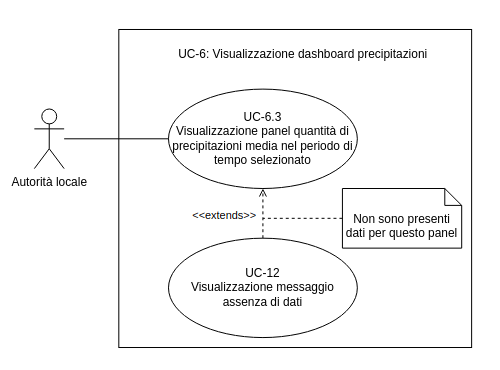
\includegraphics[width=0.75\textwidth]{analisi_dei_requisiti/UC-6.3.png}
	\captionof{figure}{UC-6.3: Visualizzazione \textit{panel} numero di veicoli in tempo reale}
\end{center}

\subsubsubsection{UC-6.4: Visualizzazione \textit{panel} velocità media in tempo reale}
\begin{itemize}
	\item \textbf{Attore principale}: Autorità locale;
	\item \textbf{Precondizioni}:
	      \begin{enumerate}
		      \item L'autorità locale ha effettuato l'accesso al sistema ed esso è in funzione;
		      \item Il sistema ha caricato la dashboard relativa ai sensori di traffico;
	      \end{enumerate}
	\item \textbf{Postcondizioni}: L'autorità locale visualizza un \textit{panel} contenente la velocità media in tempo reale;
	\item \textbf{Scenario principale}:
	      \begin{enumerate}
		      \item L'autorità locale accede alla piattaforma;
		      \item Il sistema carica i dati relativi ai sensori interrogando il database;
		      \item L'autorità locale seleziona la visualizzazione della dashboard relativa ai sensori di traffico.
	      \end{enumerate}
	\item \href{https://7last.github.io/docs/rtb/documentazione-interna/glossario\#user-story}{\textbf{User story}\textsubscript{G}}:
	      Come autorità locale desidero poter visualizzare della velocità media in tempo reale in modo da poterne monitorare l'andamento
	      e poterla facilmente confrontare con i dati storici.
\end{itemize}
\begin{center}
	
\includegraphics[width=0.75\textwidth]{analisi_dei_requisiti/UC-6.4.png}
	\captionof{figure}{UC-6.4: Visualizzazione \textit{panel} velocità media in tempo reale}
\end{center}

\subsubsubsection{UC-6.5: Visualizzazione \textit{panel} calcolo ora di punta}
\begin{itemize}
	\item \textbf{Attore principale}: Autorità locale;
	\item \textbf{Precondizioni}:
	      \begin{enumerate}
		      \item L'autorità locale ha effettuato l'accesso al sistema ed esso è in funzione;
		      \item Il sistema ha caricato la dashboard relativa ai sensori di traffico;
	      \end{enumerate}
	\item \textbf{Postcondizioni}: L'autorità locale visualizza un \textit{panel} contenente il calcolo dell'ora di punta basato sul numero di veicoli e sulla velocità media;
	\item \textbf{Scenario principale}:
	      \begin{enumerate}
		      \item L'autorità locale accede alla piattaforma;
		      \item Il sistema carica i dati relativi ai sensori interrogando il database;
		      \item L'autorità locale seleziona la visualizzazione della dashboard relativa ai sensori di traffico.
	      \end{enumerate}
	\item \href{https://7last.github.io/docs/rtb/documentazione-interna/glossario\#user-story}{\textbf{User story}\textsubscript{G}}:
	      Come autorità locale desidero poter visualizzare il calcolo dell'ora di punta basato sul numero di veicoli e sulla velocità media in modo da poter monitorare
	      l'andamento del traffico e poterlo confrontare con i dati storici.
\end{itemize}
\begin{center}
	
\includegraphics[width=0.75\textwidth]{analisi_dei_requisiti/UC-6.5.png}
	\captionof{figure}{UC-6.5: Visualizzazione \textit{panel} calcolo ora di punta}
\end{center}


\subsubsection{UC-7: Visualizzazione dashboard colonnine di ricarica}
\begin{itemize}
	\item \textbf{Attore principale}: Autorità locale;
	\item \textbf{Precondizioni}: L'autorità locale ha effettuato l'accesso al sistema ed esso è in funzione;
	\item \textbf{Postcondizioni}: L'autorità locale visualizza la dashboard relativa
	      alle colonnine di ricarica presenti nella città;
	\item \textbf{Scenario principale}:
	      \begin{enumerate}
		      \item L'autorità locale accede alla piattaforma;
		      \item Il sistema carica i dati trasmessi dai sensori interrogando il database;
		      \item L'autorità locale seleziona la visualizzazione della dashboard relativa alle colonnine di ricarica.
	      \end{enumerate}
	\item \href{https://7last.github.io/docs/rtb/documentazione-interna/glossario\#user-story}{\textbf{User story}\textsubscript{G}}:
	      Come autorità locale desidero poter visualizzare una dashboard relativa alle colonnine di ricarica presenti nella città, la quale
	      dovrà contenere informazioni riguro il loro stato di funzionamento e manutenzione.
\end{itemize}
\begin{center}
	
\includegraphics[width=0.6\textwidth]{analisi_dei_requisiti/UC-7.png}
	\captionof{figure}{UC-7: Visualizzazione dashboard colonnine di ricarica}
\end{center}

\subsubsubsection{UC-7.1: Visualizzazione mappa colonnine di ricarica con stato}
\begin{itemize}
	\item \textbf{Attore principale}: Autorità locale;
	\item \textbf{Precondizioni}:
	      \begin{enumerate}
		      \item L'autorità locale ha effettuato l'accesso al sistema ed esso è in funzione;
		      \item Il sistema ha caricato la dashboard relativa alle colonnine di ricarica;
	      \end{enumerate}
	\item \textbf{Postcondizioni}: L'autorità locale visualizza una mappa interattiva popolata con dei marker rappresentanti la posizione delle colonnine di ricarica;
	\item \textbf{Scenario principale}:
	      \begin{enumerate}
		      \item L'autorità locale accede alla piattaforma;
		      \item Il sistema carica i dati relativi ai sensori interrogando il database;
		      \item L'autorità locale seleziona la visualizzazione della dashboard relativa delle colonnine di ricarica.
	      \end{enumerate}
	\item \href{https://7last.github.io/docs/rtb/documentazione-interna/glossario\#user-story}{\textbf{User story}\textsubscript{G}}:
	      Come autorità locale desidero poter visualizzare una mappa interattiva popolata con dei marker rappresentanti la posizione delle colonnine di ricarica
	      contenenti il loro identificativo e lo stato di funzionamento. Essa mi consentirà di visualizzare la distribuzione delle colonnine di ricarica nel territorio
	      ed eventualmente interventire nel caso in cui vi siano dei guasti.
\end{itemize}
\begin{center}
	
\includegraphics[width=0.75\textwidth]{analisi_dei_requisiti/UC-7.1.png}
	\captionof{figure}{UC-7.1: Visualizzazione mappa interattiva sensori colonnine di ricarica}
\end{center}

\subsubsubsection{UC-7.2: Visualizzazione \textit{panel} numero colonnine di ricarica per stato in tempo reale}
\begin{itemize}
	\item \textbf{Attore principale}: Autorità locale;
	\item \textbf{Precondizioni}:
	      \begin{enumerate}
		      \item L'autorità locale ha effettuato l'accesso al sistema ed esso è in funzione;
		      \item Il sistema ha caricato la dashboard relativa ai dati atmosferici;
	      \end{enumerate}
	\item \textbf{Postcondizioni}: L'autorità locale visualizza un \textit{panel} contenente il conteggio delle colonnine di ricarica suddivise per stato di funzionamento;
	\item \textbf{Scenario principale}:
	      \begin{enumerate}
		      \item L'autorità locale accede alla piattaforma;
		      \item Il sistema carica i dati relativi ai sensori interrogando il database;
		      \item L'autorità locale seleziona la visualizzazione della dashboard relativa alle colonnine di ricarica.
	      \end{enumerate}
	\item \href{https://7last.github.io/docs/rtb/documentazione-interna/glossario\#user-story}{\textbf{User story}\textsubscript{G}}:
	      Come autorità locale desidero poter visualizzare un \textit{panel} contenente il conteggio delle colonnine di ricarica suddivise per stato di funzionamento
	      per poterle monitorare e intervenire in caso di guasti.
\end{itemize}
\begin{center}
	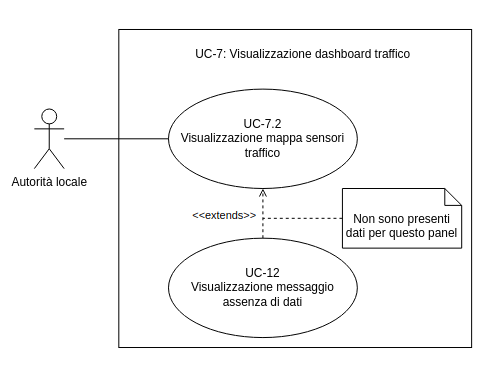
\includegraphics[width=0.6\textwidth]{analisi_dei_requisiti/UC-7.2.png}
	\captionof{figure}{UC-7.2: Visualizzazione \textit{panel} numero colonnine di ricarica per stato}
\end{center}

\subsubsection{UC-8: Visualizzazione dashboard parcheggi}
\begin{itemize}
	\item \textbf{Attore principale}: Autorità locale;
	\item \textbf{Precondizioni}: L'autorità locale ha effettuato l'accesso al sistema ed esso è in funzione;
	\item \textbf{Postcondizioni}: L'autorità locale visualizza la dashboard relativa
	      ai parcheggi presenti nella città;
	\item \textbf{Scenario principale}:
	      \begin{enumerate}
		      \item L'autorità locale accede alla piattaforma;
		      \item Il sistema carica i dati trasmessi dai sensori interrogando il database;
		      \item L'autorità locale seleziona la visualizzazione della dashboard relativa ai parcheggi.
	      \end{enumerate}
	\item \href{https://7last.github.io/docs/rtb/documentazione-interna/glossario\#user-story}{\textbf{User story}\textsubscript{G}}:
	      Come autorità locale desidero poter visualizzare una dashboard relativa ai parcheggi presenti nella città, la quale
	      dovrà contenere informazioni utili per monitorare lo stato di occupazione dei parcheggi sulla base di dati storici e in tempo reale,
	      in modo da poter individuare eventuali zone di criticità e intervenire per aumentare la disponibilità di parcheggi.
\end{itemize}
\begin{center}
	
\includegraphics[width=0.6\textwidth]{analisi_dei_requisiti/UC-8.png}
	\captionof{figure}{UC-8: Visualizzazione dashboard parcheggi}
\end{center}

\subsubsubsection{UC-8.1: Visualizzazione mappa interattiva parcheggi con rispettivo stato di occupazione}
\begin{itemize}
	\item \textbf{Attore principale}: Autorità locale;
	\item \textbf{Precondizioni}:
	      \begin{enumerate}
		      \item L'autorità locale ha effettuato l'accesso al sistema ed esso è in funzione;
		      \item Il sistema ha caricato la dashboard relativa ai parcheggi con rispettivo stato di occupazione;
	      \end{enumerate}
	\item \textbf{Postcondizioni}: L'autorità locale visualizza una mappa interattiva popolata con dei marker rappresentanti la posizione dei parcheggi con rispettivo stato di occupazione;
	\item \textbf{Scenario principale}:
	      \begin{enumerate}
		      \item L'autorità locale accede alla piattaforma;
		      \item Il sistema carica i dati relativi ai sensori interrogando il database;
		      \item L'autorità locale seleziona la visualizzazione della dashboard relativa ai parcheggi.
	      \end{enumerate}
	\item \href{https://7last.github.io/docs/rtb/documentazione-interna/glossario\#user-story}{\textbf{User story}\textsubscript{G}}:
	      Come autorità locale desidero poter visualizzare una mappa interattiva popolata con dei marker rappresentanti la posizione dei parcheggi con rispettivo stato di occupazione
	      e contenenti il loro identificativo. Essa consentirà di individuare facilmente le zone con maggiore affluenza ed eventualmente intervenire per aumentare la disponibilità di parcheggi.
\end{itemize}
\begin{center}
	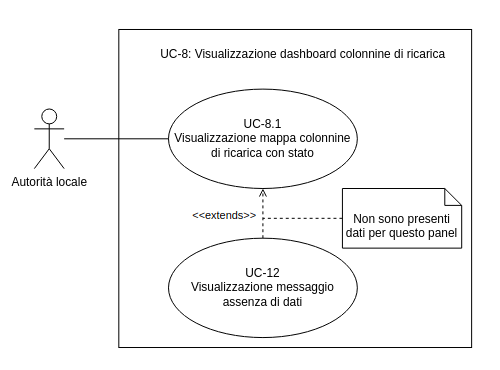
\includegraphics[width=0.75\textwidth]{analisi_dei_requisiti/UC-8.1.png}
	\captionof{figure}{UC-8.1: Visualizzazione mappa interattiva sensori parcheggi con rispettivo stato di occupazione}
\end{center}

\subsubsubsection{UC-8.2: Visualizzazione \textit{panel} con conteggio parcheggi per stato in tempo reale}
\begin{itemize}
	\item \textbf{Attore principale}: Autorità locale;
	\item \textbf{Precondizioni}:
	      \begin{enumerate}
		      \item L'autorità locale ha effettuato l'accesso al sistema ed esso è in funzione;
		      \item Il sistema ha caricato la dashboard relativa ai parcheggi;
	      \end{enumerate}
	\item \textbf{Postcondizioni}: L'autorità locale visualizza un \textit{panel} contenente i parcheggi con rispettivo stato di occupazione in tempo reale;
	\item \textbf{Scenario principale}:
	      \begin{enumerate}
		      \item L'autorità locale accede alla piattaforma;
		      \item Il sistema carica i dati relativi ai sensori interrogando il database;
		      \item L'autorità locale seleziona la visualizzazione della dashboard relativa ai parcheggi con rispettivo stato di occupazione.
	      \end{enumerate}
	\item \href{https://7last.github.io/docs/rtb/documentazione-interna/glossario\#user-story}{\textbf{User story}\textsubscript{G}}:
	      Come autorità locale desidero poter visualizzare i parcheggi con rispettivo stato di occupazione in tempo reale in modo da poterne monitorare l'andamento
	      e poterla facilmente confrontare con i dati storici.
\end{itemize}
\begin{center}
	
\includegraphics[width=0.75\textwidth]{analisi_dei_requisiti/UC-8.2.png}
	\captionof{figure}{UC-8.2: Visualizzazione \textit{panel} parcheggi con rispettivo stato di occupazione in tempo reale}
\end{center}

\subsubsection{UC-9: Visualizzazione dashboard isole ecologiche}
\begin{itemize}
	\item \textbf{Attore principale}: Autorità locale;
	\item \textbf{Precondizioni}: L'autorità locale ha effettuato l'accesso al sistema ed esso è in funzione;
	\item \textbf{Postcondizioni}: L'autorità locale visualizza la dashboard relativa
	      alle isole ecologiche presenti nella città;
	\item \textbf{Scenario principale}:
	      \begin{enumerate}
		      \item L'autorità locale accede alla piattaforma;
		      \item Il sistema carica i dati trasmessi dai sensori interrogando il database;
		      \item L'autorità locale seleziona la visualizzazione della dashboard relativa alle isole ecologiche.
	      \end{enumerate}
	\item \href{https://7last.github.io/docs/rtb/documentazione-interna/glossario\#user-story}{\textbf{User story}\textsubscript{G}}:
	      Come autorità locale desidero poter visualizzare una dashboard relativa alle isole ecologiche presenti nella città, la quale
	      dovrà contenere informazioni utili per monitorare il loro stato di riempimento. In questo modo potrò intervenire
	      per poter svuotare le isole ecologiche piene.
\end{itemize}
\begin{center}
	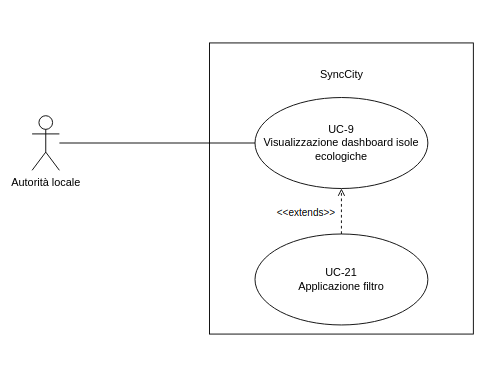
\includegraphics[width=0.6\textwidth]{analisi_dei_requisiti/UC-9.png}
	\captionof{figure}{UC-9: Visualizzazione dashboard isole ecologiche}
\end{center}

\subsubsubsection{UC-9.1: Visualizzazione \textit{panel} con conteggio isole ecologiche piene in tempo reale}
\begin{itemize}
	\item \textbf{Attore principale}: Autorità locale;
	\item \textbf{Precondizioni}:
	      \begin{enumerate}
		      \item L'autorità locale ha effettuato l'accesso al sistema ed esso è in funzione;
		      \item Il sistema ha caricato la dashboard relativa alle isole ecologiche;
	      \end{enumerate}
	\item \textbf{Postcondizioni}: L'autorità locale visualizza un \textit{panel} contenente un conteggio delle isole ecologiche piene in tempo reale;
	\item \textbf{Scenario principale}:
	      \begin{enumerate}
		      \item L'autorità locale accede alla piattaforma;
		      \item Il sistema carica i dati relativi ai sensori interrogando il database;
		      \item L'autorità locale seleziona la visualizzazione della dashboard relativa alle isole ecologiche.
	      \end{enumerate}
	\item \href{https://7last.github.io/docs/rtb/documentazione-interna/glossario\#user-story}{\textbf{User story}\textsubscript{G}}:
	      Come autorità locale desidero poter visualizzare un conteggio delle isole ecologiche piene in tempo reale in modo da poter intervenire
	      per svuotarle.
\end{itemize}
\begin{center}
	
\includegraphics[width=0.75\textwidth]{analisi_dei_requisiti/UC-9.1.png}
	\captionof{figure}{UC-9.1: Visualizzazione \textit{panel} isole ecologiche piene in tempo reale}
\end{center}

\subsubsubsection{UC-9.2: Visualizzazione mappa interattiva isole ecologiche per stato di riempimento}
\begin{itemize}
	\item \textbf{Attore principale}: Autorità locale;
	\item \textbf{Precondizioni}:
	      \begin{enumerate}
		      \item L'autorità locale ha effettuato l'accesso al sistema ed esso è in funzione;
		      \item Il sistema ha caricato la dashboard relativa ai sensori di isole ecologiche;
	      \end{enumerate}
	\item \textbf{Postcondizioni}: L'autorità locale visualizza una mappa interattiva popolata con dei marker rappresentanti la posizione dei sensori delle isole ecologiche
	      suddivise per stato di riempimento;
	\item \textbf{Scenario principale}:
	      \begin{enumerate}
		      \item L'autorità locale accede alla piattaforma;
		      \item Il sistema carica i dati relativi ai sensori interrogando il database;
		      \item L'autorità locale seleziona la visualizzazione della dashboard relativa ai sensori delle isole ecologiche piene.
	      \end{enumerate}
	\item \href{https://7last.github.io/docs/rtb/documentazione-interna/glossario\#user-story}{\textbf{User story}\textsubscript{G}}:
	      Come autorità locale desidero poter visualizzare una mappa interattiva popolata con dei marker rappresentanti la posizione dei sensori delle isole ecologiche
	      suddivise per stato di riempimento e contenenti il loro identificativo.
	      Essa mi consentirà di visualizzare la distribuzione delle isole ecologiche nel territorio e di individuare facilmente quelle piene per poter intervenire e svuotarle.
\end{itemize}
\begin{center}
	
\includegraphics[width=0.75\textwidth]{analisi_dei_requisiti/UC-9.2.png}
	\captionof{figure}{UC-9.2: Visualizzazione mappa interattiva sensori isole ecologiche piene}
\end{center}

\subsubsection{UC-10: Visualizzazione dashboard livello di acqua}
\begin{itemize}
	\item \textbf{Attore principale}: Autorità locale;
	\item \textbf{Precondizioni}: L'autorità locale ha effettuato l'accesso al sistema ed esso è in funzione;
	\item \textbf{Postcondizioni}: L'autorità locale visualizza la dashboard relativa
	      ai sensori del livello di acqua presenti nella città;
	\item \textbf{Scenario principale}:
	      \begin{enumerate}
		      \item L'autorità locale accede alla piattaforma;
		      \item Il sistema carica i dati trasmessi dai sensori interrogando il database;
		      \item L'autorità locale seleziona la visualizzazione della dashboard relativa ai sensori del livello di acqua.
	      \end{enumerate}
	\item \href{https://7last.github.io/docs/rtb/documentazione-interna/glossario\#user-story}{\textbf{User story}\textsubscript{G}}:
	      Come autorità locale desidero poter visualizzare una dashboard relativa ai sensori del livello di acqua presenti nella città, la quale
	      dovrà contenere informazioni utili per monitorare il livello di acqua sulla base di dati storici e in tempo reale, mostrando
	      anche statistiche quali del livello di acqua medio nel periodo di tempo selezionato e il livello di acqua in tempo reale.
\end{itemize}
\begin{center}
	\includegraphics[width=0.6\textwidth]{analisi_dei_requisiti/UC-10.png}
	\captionof{figure}{UC-10: Visualizzazione dashboard livello di acqua}
\end{center}

\subsubsubsection{UC-10.1: Visualizzazione grafico time series livello di acqua}
\begin{itemize}
	\item \textbf{Attore principale}: Autorità locale;
	\item \textbf{Precondizioni}:
	      \begin{enumerate}
		      \item L'autorità locale ha effettuato l'accesso al sistema ed esso è in funzione;
		      \item Il sistema ha caricato la dashboard relativa ai sensori del livello di acqua.
	      \end{enumerate}
	\item \textbf{Postcondizioni}: L'autorità locale visualizza un grafico time series contenente le misurazioni storiche
	      del livello di acqua aggregate per 5 minuti;
	\item \textbf{Scenario principale}:
	      \begin{enumerate}
		      \item L'autorità locale accede alla piattaforma;
		      \item Il sistema carica i dati relativi ai sensori interrogando il database;
		      \item L'autorità locale seleziona la visualizzazione della dashboard relativa ai sensori del livello di acqua;
	      \end{enumerate}
	\item \href{https://7last.github.io/docs/rtb/documentazione-interna/glossario\#user-story}{\textbf{User story}\textsubscript{G}}:
	      Come autorità locale desidero poter visualizzare un grafico time series contenente le misurazioni storiche
	      del livello di acqua per poter monitorarne l'andamento nel tempo e facilmente individuare eventuali anomalie.
\end{itemize}
\begin{center}
	\includegraphics[width=0.75\textwidth]{analisi_dei_requisiti/UC-10.1.png}
	\captionof{figure}{UC-10.1, Visualizzazione grafico time series livello di acqua}
\end{center}

\subsubsubsection{UC-10.2: Visualizzazione mappa sensori livello di acqua}
\begin{itemize}
	\item \textbf{Attore principale}: Autorità locale;
	\item \textbf{Precondizioni}:
	      \begin{enumerate}
		      \item L'autorità locale ha effettuato l'accesso al sistema ed esso è in funzione;
		      \item Il sistema ha caricato la dashboard relativa ai sensori del livello di acqua;
	      \end{enumerate}
	\item \textbf{Postcondizioni}: L'autorità locale visualizza una mappa interattiva popolata con dei marker rappresentanti la posizione dei sensori del livello di acqua;
	\item \textbf{Scenario principale}:
	      \begin{enumerate}
		      \item L'autorità locale accede alla piattaforma;
		      \item Il sistema carica i dati relativi ai sensori interrogando il database;
		      \item L'autorità locale seleziona la visualizzazione della dashboard relativa ai sensori del livello di acqua.
	      \end{enumerate}
	\item \href{https://7last.github.io/docs/rtb/documentazione-interna/glossario\#user-story}{\textbf{User story}\textsubscript{G}}:
	      Come autorità locale desidero poter visualizzare una mappa interattiva popolata con dei marker rappresentanti la posizione dei sensori del livello di acqua
	      e contenenti il loro identificativo. Essa mi consentirà di visualizzare la distribuzione dei sensori del livello di acqua nel territorio ed eventualmente interventire nel caso in cui siano presenti zone non coperte.
\end{itemize}
\begin{center}
	\includegraphics[width=0.75\textwidth]{analisi_dei_requisiti/UC-10.2.png}
	\captionof{figure}{UC-10.2: Visualizzazione mappa interattiva sensori livello di acqua}
\end{center}

\subsubsubsection{UC-10.3: Visualizzazione \textit{panel} livello di acqua medio nel periodo di tempo selezionato}
\begin{itemize}
	\item \textbf{Attore principale}: Autorità locale;
	\item \textbf{Precondizioni}:
	      \begin{enumerate}
		      \item L'autorità locale ha effettuato l'accesso al sistema ed esso è in funzione;
		      \item Il sistema ha caricato la dashboard relativa ai sensori di livello di acqua;
	      \end{enumerate}
	\item \textbf{Postcondizioni}: L'autorità locale visualizza un \textit{panel} contenente del livello di acqua medio nel periodo di tempo selezionato;
	\item \textbf{Scenario principale}:
	      \begin{enumerate}
		      \item L'autorità locale accede alla piattaforma;
		      \item Il sistema carica i dati relativi ai sensori interrogando il database;
		      \item L'autorità locale seleziona la visualizzazione della dashboard relativa ai sensori di livello di acqua.
	      \end{enumerate}
	\item \href{https://7last.github.io/docs/rtb/documentazione-interna/glossario\#user-story}{\textbf{User story}\textsubscript{G}}:
	      Come autorità locale desidero poter visualizzare del livello di acqua medio nel periodo di tempo selezionato
	      in modo da poterne monitorare l'andamento.
\end{itemize}
\begin{center}
	\includegraphics[width=0.75\textwidth]{analisi_dei_requisiti/UC-10.3.png}
	\captionof{figure}{UC-10.3: Visualizzazione \textit{panel} livello di acqua medio nel periodo di tempo selezionato}
\end{center}

\subsubsubsection{UC-10.4: Visualizzazione \textit{panel} livello di acqua in tempo reale}
\begin{itemize}
	\item \textbf{Attore principale}: Autorità locale;
	\item \textbf{Precondizioni}:
	      \begin{enumerate}
		      \item L'autorità locale ha effettuato l'accesso al sistema ed esso è in funzione;
		      \item Il sistema ha caricato la dashboard relativa ai sensori di livello di acqua;
	      \end{enumerate}
	\item \textbf{Postcondizioni}: L'autorità locale visualizza un \textit{panel} contenente il livello di acqua in tempo reale;
	\item \textbf{Scenario principale}:
	      \begin{enumerate}
		      \item L'autorità locale accede alla piattaforma;
		      \item Il sistema carica i dati relativi ai sensori interrogando il database;
		      \item L'autorità locale seleziona la visualizzazione della dashboard relativa ai sensori di livello di acqua.
	      \end{enumerate}
	\item \href{https://7last.github.io/docs/rtb/documentazione-interna/glossario\#user-story}{\textbf{User story}\textsubscript{G}}:
	      Come autorità locale desidero poter visualizzare il livello di acqua in tempo reale in modo da poterne monitorare l'andamento
	      e poterlo facilmente confrontare con i dati storici.
\end{itemize}
\begin{center}
	\includegraphics[width=0.75\textwidth]{analisi_dei_requisiti/UC-10.4.png}
	\captionof{figure}{UC-10.4: Visualizzazione \textit{panel} livello di acqua in tempo reale}
\end{center}

\subsubsection{UC-11: Visualizzazione messaggio assenza di dati}
\begin{itemize}
	\item \textbf{Attore principale}: Autorità locale;
	\item \textbf{Precondizioni}:
	      \begin{enumerate}
		      \item L'autorità locale accede alla piattaforma;
		      \item Il sistema carica i dati relativi ai sensori interrogando il database;
	      \end{enumerate}
	\item \textbf{Postcondizioni}: L'autorità locale visualizza un messaggio che notifica l'assenza di dati;
	\item \textbf{Scenario principale}:
	      \begin{enumerate}
		      \item L'autorità locale accede alla piattaforma;
		      \item Il sistema carica i dati relativi ai sensori interrogando il database;
		      \item Il sistema non trova dati relativi ai sensori;
		      \item Il sistema mostra un messaggio che notifica l'assenza di dati.
	      \end{enumerate}
\end{itemize}

\subsubsection{UC-12: Trasmissione dati temperatura}
\begin{itemize}
	\item \textbf{Attore principale}: Sensore;
	\item \textbf{Precondizioni}: Il sensore è attivo e collegato al sistema;
	\item \textbf{Postcondizioni}: I dati inviati dal sensore sono stati elaborati e memorizzati nel sistema;
	\item \textbf{Scenario principale}:
	      \begin{enumerate}
		      \item Il sensore effettua una misurazione di temperatura;
		      \item Il sensore formatta i dati da inviare al sistema, includendo oltre alle misurazioni l'identificativo del sensore,
		            il timestamp, e la sua posizione geografica;
		      \item Il sensore invia i dati al sistema.
	      \end{enumerate}
	\item \href{https://7last.github.io/docs/rtb/documentazione-interna/glossario\#user-story}{\textbf{User story}\textsubscript{G}}: Come sensore, desidero poter inviare al sistema le rilevazioni della temperatura.
\end{itemize}

\begin{center}
	\includegraphics[width=0.6\textwidth]{analisi_dei_requisiti/UC-12.png}
	\captionof{figure}{UC-12: Trasmissione dati temperatura}
\end{center}

\subsubsection{UC-13: Trasmissione dati umidità}
\begin{itemize}
	\item \textbf{Attore principale}: Sensore;
	\item \textbf{Precondizioni}: Il sensore è attivo e collegato al sistema;
	\item \textbf{Postcondizioni}: I dati inviati dal sensore sono stati elaborati e memorizzati nel sistema;
	\item \textbf{Scenario principale}:
	      \begin{enumerate}
		      \item Il sensore effettua una misurazione dell'umidità;
		      \item Il sensore formatta i dati da inviare al sistema, includendo oltre alle misurazioni l'identificativo del sensore,
		            il timestamp, e la sua posizione geografica;
		      \item Il sensore invia i dati al sistema.
	      \end{enumerate}
	\item \href{https://7last.github.io/docs/rtb/documentazione-interna/glossario\#user-story}{\textbf{User story}\textsubscript{G}}: Come sensore, desidero poter inviare al sistema le rilevazioni dell'umidità.
\end{itemize}

\begin{center}
	\includegraphics[width=0.6\textwidth]{analisi_dei_requisiti/UC-13.png}
	\captionof{figure}{UC-13: Trasmissione dati umidità}
\end{center}

\subsubsection{UC-14: Trasmissione dati qualità dell'aria}
\begin{itemize}
	\item \textbf{Attore principale}: Sensore;
	\item \textbf{Precondizioni}: Il sensore è attivo e collegato al sistema;
	\item \textbf{Postcondizioni}: I dati inviati dal sensore sono stati elaborati e memorizzati nel sistema;
	\item \textbf{Scenario principale}:
	      \begin{enumerate}
		      \item Il sensore effettua una misurazione della quantità di precipitazioni;
		      \item Il sensore formatta i dati da inviare al sistema, includendo oltre alle misurazioni l'identificativo del sensore,
		            il timestamp, e la sua posizione geografica;
		      \item Il sensore invia i dati al sistema.
	      \end{enumerate}
	\item \href{https://7last.github.io/docs/rtb/documentazione-interna/glossario\#user-story}{\textbf{User story}\textsubscript{G}}:
	      Come sensore, desidero poter inviare al sistema le rilevazioni della qualità dell'aria.
\end{itemize}

\begin{center}
	\includegraphics[width=0.6\textwidth]{analisi_dei_requisiti/UC-14.png}
	\captionof{figure}{UC-14: Trasmissione dati precipitazioni}
\end{center}

\subsubsection{UC-15: Trasmissione dati precipitazioni}
\begin{itemize}
	\item \textbf{Attore principale}: Sensore;
	\item \textbf{Precondizioni}: Il sensore è attivo e collegato al sistema;
	\item \textbf{Postcondizioni}: I dati inviati dal sensore sono stati elaborati e memorizzati nel sistema;
	\item \textbf{Scenario principale}:
	      \begin{enumerate}
		      \item Il sensore effettua una misurazione della quantità di precipitazioni;
		      \item Il sensore formatta i dati da inviare al sistema, includendo oltre alle misurazioni l'identificativo del sensore,
		            il timestamp, e la sua posizione geografica;
		      \item Il sensore invia i dati al sistema.
	      \end{enumerate}
	\item \href{https://7last.github.io/docs/rtb/documentazione-interna/glossario\#user-story}{\textbf{User story}\textsubscript{G}}: Come sensore, desidero poter inviare al sistema le rilevazioni della quantità di precipitazioni.
\end{itemize}

\begin{center}
	\includegraphics[width=0.6\textwidth]{analisi_dei_requisiti/UC-15.png}
	\captionof{figure}{UC-15: Trasmissione dati precipitazioni}
\end{center}

\subsubsection{UC-16: Trasmissione dati traffico}
\begin{itemize}
	\item \textbf{Attore principale}: Sensore;
	\item \textbf{Precondizioni}: Il sensore è attivo e collegato al sistema;
	\item \textbf{Postcondizioni}: I dati inviati dal sensore sono stati elaborati e memorizzati nel sistema;
	\item \textbf{Scenario principale}:
	      \begin{enumerate}
		      \item Il sensore effettua una misurazione del traffico;
		      \item Il sensore formatta i dati da inviare al sistema, includendo oltre alle misurazioni l'identificativo del sensore,
		            il timestamp, e la sua posizione geografica;
		      \item Il sensore invia i dati al sistema.
	      \end{enumerate}
	\item \href{https://7last.github.io/docs/rtb/documentazione-interna/glossario\#user-story}{\textbf{User story}\textsubscript{G}}: Come sensore, desidero poter inviare al sistema le rilevazioni sui dati del traffico.
\end{itemize}

\begin{center}
	\includegraphics[width=0.6\textwidth]{analisi_dei_requisiti/UC-16.png}
	\captionof{figure}{UC-16: Trasmissione dati traffico}
\end{center}


\subsubsection{UC-17: Trasmissione dati colonnine di ricarica}
\begin{itemize}
	\item \textbf{Attore principale}: Sensore;
	\item \textbf{Precondizioni}: Il sensore è attivo e collegato al sistema;
	\item \textbf{Postcondizioni}: I dati inviati dal sensore sono stati elaborati e memorizzati nel sistema;
	\item \textbf{Scenario principale}:
	      \begin{enumerate}
		      \item Il sensore effettua una misurazione dello stato e l'occupazione delle colonnine di ricarica;
		      \item Il sensore formatta i dati da inviare al sistema, includendo oltre alle misurazioni l'identificativo del sensore,
		            il timestamp, e la sua posizione geografica;
		      \item Il sensore invia i dati al sistema.
	      \end{enumerate}
	\item \href{https://7last.github.io/docs/rtb/documentazione-interna/glossario\#user-story}{\textbf{User story}\textsubscript{G}}: Come sensore, desidero poter inviare al sistema le rilevazioni sullo stato e l'occupazione delle colonnine di ricarica.
\end{itemize}
\begin{center}
	\includegraphics[width=0.6\textwidth]{analisi_dei_requisiti/UC-17.png}
	\captionof{figure}{UC-17: Trasmissione dati colonnine di ricarica}
\end{center}

\subsubsection{UC-18: Trasmissione dati parcheggi}
\begin{itemize}
	\item \textbf{Attore principale}: Sensore;
	\item \textbf{Precondizioni}: Il sensore è attivo e collegato al sistema;
	\item \textbf{Postcondizioni}: I dati inviati dal sensore sono stati elaborati e memorizzati nel sistema;
	\item \textbf{Scenario principale}:
	      \begin{enumerate}
		      \item Il sensore effettua una misurazione dello stato di riempimento del parcheggio;
		      \item Il sensore formatta i dati da inviare al sistema, includendo oltre alle misurazioni l'identificativo del sensore,
		            il timestamp, e la sua posizione geografica;
		      \item Il sensore invia i dati al sistema.
	      \end{enumerate}
	\item \href{https://7last.github.io/docs/rtb/documentazione-interna/glossario\#user-story}{\textbf{User story}\textsubscript{G}}: Come sensore, desidero poter inviare al sistema le rilevazioni sull'occupazione dei parcheggi.
\end{itemize}

\begin{center}
	\includegraphics[width=0.6\textwidth]{analisi_dei_requisiti/UC-18.png}
	\captionof{figure}{UC-18: Trasmissione dati parcheggi}
\end{center}

\subsubsection{UC-19: Trasmissione dati isole ecologiche}
\begin{itemize}
	\item \textbf{Attore principale}: Sensore;
	\item \textbf{Precondizioni}: Il sensore è attivo e collegato al sistema;
	\item \textbf{Postcondizioni}: I dati inviati dal sensore sono stati elaborati e memorizzati nel sistema;
	\item \textbf{Scenario principale}:
	      \begin{enumerate}
		      \item Il sensore effettua una misurazione dello stato di riempimento delle isole ecologiche;
		      \item Il sensore formatta i dati da inviare al sistema, includendo oltre alle misurazioni l'identificativo del sensore,
		            il timestamp, e la sua posizione geografica;
		      \item Il sensore invia i dati al sistema.
	      \end{enumerate}
	\item \href{https://7last.github.io/docs/rtb/documentazione-interna/glossario\#user-story}{\textbf{User story}\textsubscript{G}}: Come sensore, desidero poter inviare al sistema le rilevazioni sullo stato di riempimento delle isole ecologiche.
\end{itemize}

\begin{center}
	\includegraphics[width=0.6\textwidth]{analisi_dei_requisiti/UC-19.png}
	\captionof{figure}{UC-19: Trasmissione dati isole ecologiche}
\end{center}

\subsubsection{UC-20: Trasmissione dati livello di acqua}
\begin{itemize}
	\item \textbf{Attore principale}: Sensore;
	\item \textbf{Precondizioni}: Il sensore è attivo e collegato al sistema;
	\item \textbf{Postcondizioni}: I dati inviati dal sensore sono stati elaborati e memorizzati nel sistema;
	\item \textbf{Scenario principale}:
	      \begin{enumerate}
		      \item Il sensore effettua una misurazione del livello di acqua;
		      \item Il sensore formatta i dati da inviare al sistema, includendo oltre alle misurazioni l'identificativo del sensore,
		            il timestamp, e la sua posizione geografica;
		      \item Il sensore invia i dati al sistema.
	      \end{enumerate}
	\item \href{https://7last.github.io/docs/rtb/documentazione-interna/glossario\#user-story}{\textbf{User story}\textsubscript{G}}: Come sensore, desidero poter inviare al sistema le rilevazioni sul livello di acqua.
\end{itemize}

\begin{center}
	\includegraphics[width=0.6\textwidth]{analisi_dei_requisiti/UC-20.png}
	\captionof{figure}{UC-20: Trasmissione dati livello di acqua}
\end{center}

\subsubsection{UC-21: Applicazione filtro sensore}
\begin{itemize}
	\item \textbf{Attore principale}: Autorità locale;
	\item \textbf{Precondizioni}:
	      \begin{enumerate}
		      \item L'autorità locale ha effettuato l'accesso al sistema ed esso è in funzione;
		      \item Il sistema ha caricato i dati interrogando il database;
		      \item L'autorità locale visualizza una dashboard.
	      \end{enumerate}
	\item \textbf{Postcondizioni}: L'autorità locale applica un filtro ai dati visualizzati in modo da poter visualizzare solo i dati relativi ad un sensore specifico;
	\item \textbf{Scenario principale}:
	      \begin{enumerate}
		      \item L'autorità locale visualizza una dashboard;
		      \item L'autorità locale seleziona il sensore di cui vuole visualizzare i dati;
	      \end{enumerate}
	\item \href{https://7last.github.io/docs/rtb/documentazione-interna/glossario\#user-story}{\textbf{User story}\textsubscript{G}}:
	      Come autorità locale desidero poter visualizzare solo i dati relativi ad un sensore specifico in modo da poter facilmente
	      monitorare i dati di un sensore specifico e circoscrivere l'analisi ai dati di interesse.
\end{itemize}
\begin{center}
	\includegraphics[width=0.6\textwidth]{analisi_dei_requisiti/UC-21.png}
	\captionof{figure}{UC-21: Applicazione filtro sensore}
\end{center}


%---------4_PIANIFICAZIONE-----------%
\section{Requisiti}
\subsection{Definizione di un requisito}
Per ciascun requisito vengono fornite le seguenti informazioni:
\begin{itemize}
	\item \textbf{Codice}: codice identificativo del requisito, meglio specificato nella sezione \ref{sec:codifica_requisiti};
	\item \textbf{Descrizione}: breve descrizione del requisito;
	\item \textbf{Fonte}: provenienza del requisito, meglio specificata nella sezione \ref{sec:fonti_requisiti};
	\item \textbf{Importanza}: indica l'importanza del requisito, meglio specificata nella sezione \ref{sec:importanza_requisiti}.
\end{itemize}

\subsection{Tipologie di requisiti}
I requisiti possono essere di quattro tipologie:
\begin{itemize}
	\item \textbf{Funzionali}: descrivono le funzionalità del sistema;
	\item \textbf{Qualitativi}: descrivono le qualità che il sistema deve avere;
	\item \textbf{Di vincolo}: descrivono i vincoli a cui il sistema deve sottostare;
	\item \textbf{Prestazionali}: descrivono le prestazioni che il sistema deve avere.
\end{itemize}

\subsubsection{Codifica dei requisiti}
\label{sec:codifica_requisiti}
I requisiti sono codificati nel seguente modo:
\begin{center}
	\textbf{R[Tipologia]-[Codice]}
\end{center}
dove \textbf{[Codice]} è un numero progressivo che identifica univocamente il requisito
e \textbf{[Tipologia]} è una lettera che identifica la tipologia del requisito:
\begin{itemize}
	\item \textbf{F}: requisito funzionale;
	\item \textbf{Q}: requisito qualitativo;
	\item \textbf{V}: requisito di vincolo;
\end{itemize}

\subsubsection{Fonti dei requisiti}
\label{sec:fonti_requisiti}
I requisiti possono avere le seguenti fonti:
\begin{itemize}
	\item \href{https://7last.github.io/docs/rtb/documentazione-interna/glossario\#capitolato}{\textbf{Capitolato}\textsubscript{G}}: requisiti individuati a seguito dell'analisi del \href{https://7last.github.io/docs/rtb/documentazione-interna/glossario\#capitolato}{capitolato\textsubscript{G}};
	\item \textbf{Interno}: requisiti individuati durante le riunioni interne e da coloro che hanno il ruolo di analista;
	\item \textbf{Esterno}: requisiti aggiuntivi individuati in seguito a incontri con la \href{https://7last.github.io/docs/rtb/documentazione-interna/glossario\#proponente}{proponente\textsubscript{G}};
	\item \href{https://7last.github.io/docs/rtb/documentazione-interna/glossario\#piano-di-qualifica}{\textbf{Piano di Qualifica}\textsubscript{G}}: requisiti necessari per adeguare il prodotto agli standard di qualità definiti nel documento \href{https://7last.github.io/docs/rtb/documentazione-interna/glossario\#piano-di-qualifica}{\textit{Piano di Qualifica}\textsubscript{G}}.
	\item \href{https://7last.github.io/docs/rtb/documentazione-interna/glossario\#norme-di-progetto}{\textbf{Norme di Progetto}\textsubscript{G}}: requisiti necessari per adeguare il prodotto alle norme stabilite nel documento \href{https://7last.github.io/docs/rtb/documentazione-interna/glossario\#norme-di-progetto}{\textit{Norme di Progetto}\textsubscript{G}};
\end{itemize}

\subsubsection{Importanza dei requisiti}
\label{sec:importanza_requisiti}
I requisiti possono avere tre livelli di importanza:
\begin{itemize}
	\item \textbf{Obbligatorio}: requisito irrinunciabile per il \href{https://7last.github.io/docs/rtb/documentazione-interna/glossario\#committente}{committente\textsubscript{G}};
	\item \textbf{Desiderabile}: requisito non strettamente necessario, ma che porta valore aggiunto al prodotto;
	\item \textbf{Opzionale}: requisito relativo a funzionalità aggiuntive.
\end{itemize}


\subsection{Requisiti funzionali}
\begin{longtable}{|>{\centering\arraybackslash}m{0.10\textwidth}|>{\centering\arraybackslash}m{0.20\textwidth}|>{\centering\arraybackslash}m{0.20\textwidth}|>{\centering\arraybackslash}m{0.4\textwidth}|}
	\hline
	\textbf{Codice} & \textbf{Importanza} & \textbf{Fonte}                                                                                                    & \textbf{Descrizione}                                                                                                                                                                                                                                                                                                                                                                                                                                                                                 \\\hline
	\endfirsthead
	\hline
	\textbf{Codice} & \textbf{Importanza} & \textbf{Fonte}                                                                                                    & \textbf{Descrizione}                                                                                                                                                                                                                                                                                                                                                                                                                                                                                 \\\hline
	\endhead
	\hline
	RF-1            & Obbligatorio        & \href{https://7last.github.io/docs/rtb/documentazione-interna/glossario\#capitolato}{Capitolato\textsubscript{G}} & La parte \textit{IoT} dovrà essere simulata attraverso tool di generazione di informazioni random che tuttavia siano verosimili.                                                                                                                                                                                                                                                                                                                                                                     \\\hline
	RF-2            & Obbligatorio        & \href{https://7last.github.io/docs/rtb/documentazione-interna/glossario\#capitolato}{Capitolato\textsubscript{G}} & Il sistema dovrà permettere la visualizzazione dei dati in tempo reale.                                                                                                                                                                                                                                                                                                                                                                                                                              \\\hline
	RF-3            & Obbligatorio        & \href{https://7last.github.io/docs/rtb/documentazione-interna/glossario\#capitolato}{Capitolato\textsubscript{G}} & Il sistema dovrà permettere la visualizzazione dei dati storici.                                                                                                                                                                                                                                                                                                                                                                                                                                     \\\hline
	RF-4            & Obbligatorio        & \href{https://7last.github.io/docs/rtb/documentazione-interna/glossario\#capitolato}{Capitolato\textsubscript{G}} & L'utente deve poter accedere all'applicativo senza bisogno di autenticazione.                                                                                                                                                                                                                                                                                                                                                                                                                        \\\hline
	RF-5            & Obbligatorio        & \href{https://7last.github.io/docs/rtb/documentazione-interna/glossario\#capitolato}{Capitolato\textsubscript{G}} & L'utente dovrà poter visualizzare su una mappa la posizione geografica dei sensori.                                                                                                                                                                                                                                                                                                                                                                                                                  \\\hline
	RF-6            & Obbligatorio        & \href{https://7last.github.io/docs/rtb/documentazione-interna/glossario\#capitolato}{Capitolato\textsubscript{G}} & I tipi di dati che il sistema dovrà visualizzare sono: temperatura, umidità, qualità dell'aria, precipitazioni, traffico, stato delle colonnine di ricarica, stato di occupazione dei parcheggi, stato di riempimento delle isole ecologiche e livello di acqua.                                                                                                                                                                                                                                     \\\hline
	RF-7            & Obbligatorio        & \href{https://7last.github.io/docs/rtb/documentazione-interna/glossario\#capitolato}{Capitolato\textsubscript{G}} & I dati dovranno essere salvati su un database OLAP.                                                                                                                                                                                                                                                                                                                                                                                                                                                  \\\hline
	RF-8            & Obbligatorio        & \href{https://7last.github.io/docs/rtb/documentazione-interna/glossario\#capitolato}{Capitolato\textsubscript{G}} & I sensori di temperatura rilevano i dati in Celsius                                                                                                                                                                                                                                                                                                                                                                                                                                                  \\\hline
	RF-9            & Obbligatorio        & \href{https://7last.github.io/docs/rtb/documentazione-interna/glossario\#capitolato}{Capitolato\textsubscript{G}} & I sensori di umidità rilevano la percentuale di umidità nell’aria.                                                                                                                                                                                                                                                                                                                                                                                                                                   \\\hline
	RF-10           & Obbligatorio        & \href{https://7last.github.io/docs/rtb/documentazione-interna/glossario\#capitolato}{Capitolato\textsubscript{G}} & I sensori livello acqua rilevano il livello di acqua nella zona di installazione                                                                                                                                                                                                                                                                                                                                                                                                                     \\\hline
	RF-11           & Obbligatorio        & \href{https://7last.github.io/docs/rtb/documentazione-interna/glossario\#capitolato}{Capitolato\textsubscript{G}} & I dati provenienti dai sensori dovranno contenere i seguenti dati: id \href{https://7last.github.io/docs/rtb/documentazione-interna/glossario\#sensore}{sensore\textsubscript{G}}, data, ora e valore.                                                                                                                                                                                                                                                                                               \\\hline
	RF-12           & Obbligatorio        & \href{https://7last.github.io/docs/rtb/documentazione-interna/glossario\#capitolato}{Capitolato\textsubscript{G}} & Sviluppo di componenti quali \href{https://7last.github.io/docs/rtb/documentazione-interna/glossario\#widget}{widget\textsubscript{G}} e grafici per la visualizzazione dei dati nelle \href{https://7last.github.io/docs/rtb/documentazione-interna/glossario\#dashboard}{dashboard\textsubscript{G}}.                                                                                                                                                                                              \\\hline
	RF-13           & Obbligatorio        & \href{https://7last.github.io/docs/rtb/documentazione-interna/glossario\#capitolato}{Capitolato\textsubscript{G}} & Il sistema dovrà permettere la visualizzazione dei dati in tempo reale.                                                                                                                                                                                                                                                                                                                                                                                                                              \\\hline
	RF-14           & Obbligatorio        & Interno                                                                                                           & Il sistema deve permettere di visualizzare una \href{https://7last.github.io/docs/rtb/documentazione-interna/glossario\#dashboard}{dashboard\textsubscript{G}} generale con tutti i dati dei sensori.                                                                                                                                                                                                                                                                                                \\\hline
	RF-15           & Obbligatorio        & Interno                                                                                                           & Il sistema deve permettere di visualizzare una \href{https://7last.github.io/docs/rtb/documentazione-interna/glossario\#dashboard}{dashboard\textsubscript{G}} specifica per ciascuna categoria di sensori.                                                                                                                                                                                                                                                                                          \\\hline
	RF-16           & Obbligatorio        & Interno                                                                                                           & Nella \href{https://7last.github.io/docs/rtb/documentazione-interna/glossario\#dashboard}{dashboard\textsubscript{G}} generale dovranno essere presenti una tabella di tutti i sensori, una mappa interattiva, un \href{https://7last.github.io/docs/rtb/documentazione-interna/glossario\#widget}{widget\textsubscript{G}} con il conteggio totale dei sensori e una tabella contente i sensori che non stanno inviando dati da più di un giorno.                                                   \\\hline
	RF-17           & Obbligatorio        & Interno                                                                                                           & Nella \href{https://7last.github.io/docs/rtb/documentazione-interna/glossario\#dashboard}{dashboard\textsubscript{G}} della temperatura dovranno essere visualizzati: un grafico \href{https://7last.github.io/docs/rtb/documentazione-interna/glossario\#time-series}{time series\textsubscript{G}}, una mappa interattiva, la temperatura media, minima e massima di un certo periodo di tempo e la temperatura in tempo reale.                                                                    \\\hline
	RF-18           & Obbligatorio        & Interno                                                                                                           & Nella \href{https://7last.github.io/docs/rtb/documentazione-interna/glossario\#dashboard}{dashboard\textsubscript{G}} dell'umidità dovranno essere visualizzati: un grafico \href{https://7last.github.io/docs/rtb/documentazione-interna/glossario\#time-series}{time series\textsubscript{G}}, una mappa interattiva, l'umidità media, minima e massima di un certo periodo di tempo e l'umidità in tempo reale.                                                                                   \\\hline
	RF-19           & Obbligatorio        & Interno                                                                                                           & Nella \href{https://7last.github.io/docs/rtb/documentazione-interna/glossario\#dashboard}{dashboard\textsubscript{G}} della qualità dell'aria dovranno essere visualizzati: un grafico \href{https://7last.github.io/docs/rtb/documentazione-interna/glossario\#time-series}{time series\textsubscript{G}}, una mappa interattiva, la qualità media dell'aria in un certo periodo e in tempo reale, i giorni con la qualità dell'aria migliore e peggiore in un certo periodo di tempo.              \\\hline
	RF-20           & Obbligatorio        & Interno                                                                                                           & Nella \href{https://7last.github.io/docs/rtb/documentazione-interna/glossario\#dashboard}{dashboard\textsubscript{G}} delle precipitazioni dovranno essere visualizzati: un grafico \href{https://7last.github.io/docs/rtb/documentazione-interna/glossario\#time-series}{time series\textsubscript{G}}, una mappa interattiva, la quantità media di precipitazioni in un certo periodo e in tempo reale, i giorni con la quantità di precipitazioni maggiore e minore in un certo periodo di tempo. \\\hline
	RF-20           & Obbligatorio        & Interno                                                                                                           & Nella \href{https://7last.github.io/docs/rtb/documentazione-interna/glossario\#dashboard}{dashboard\textsubscript{G}} del traffico dovranno essere visualizzati: un grafico \href{https://7last.github.io/docs/rtb/documentazione-interna/glossario\#time-series}{time series\textsubscript{G}}, il numero di veicoli e la velocità media in tempo reale e il calcolo dell'ora di punta sulla base del numero di veicoli e velocità media.                                                           \\\hline
	RF-20           & Obbligatorio        & Interno                                                                                                           & Nella \href{https://7last.github.io/docs/rtb/documentazione-interna/glossario\#dashboard}{dashboard\textsubscript{G}} delle colonnine di ricarica dovranno essere visualizzati: una mappa interattiva contenente anche lo stato e il numero di colonnine di ricarica suddivise per stato in tempo reale.                                                                                                                                                                                             \\\hline
	RF-21           & Obbligatorio        & Interno                                                                                                           & Nella \href{https://7last.github.io/docs/rtb/documentazione-interna/glossario\#dashboard}{dashboard\textsubscript{G}} dei parcheggi dovranno essere visualizzati: una mappa interattiva con il rispettivo stato di occupazione e il conteggio di parcheggi suddivisi per stato di occupazione in tempo reale.                                                                                                                                                                                        \\\hline
	RF-22           & Obbligatorio        & Interno                                                                                                           & Nella \href{https://7last.github.io/docs/rtb/documentazione-interna/glossario\#dashboard}{dashboard\textsubscript{G}} delle isole ecologiche dovranno essere visualizzati: una mappa interattiva con il rispettivo stato di riempimento e il conteggio di isole ecologiche suddivise per stato di riempimento in tempo reale.                                                                                                                                                                        \\\hline
	RF-23           & Obbligatorio        & Interno                                                                                                           & Nella \href{https://7last.github.io/docs/rtb/documentazione-interna/glossario\#dashboard}{dashboard\textsubscript{G}} del livello di acqua dovranno essere visualizzati: un grafico \href{https://7last.github.io/docs/rtb/documentazione-interna/glossario\#time-series}{time series\textsubscript{G}}, una mappa interattiva, il livello medio di acqua in un certo periodo e in tempo reale.                                                                                                      \\\hline
	RF-24           & Obbligatorio        & Interno                                                                                                           & Nel caso in cui non ci siano dati visualizzabili, il sistema deve notificare l'utente mostrando un opportuno messaggio.                                                                                                                                                                                                                                                                                                                                                                              \\\hline
	RF-25           & Obbligatorio        & Interno                                                                                                           & I sensori di qualità dell'aria inviano i seguenti dati: \textit{PM10}, \textit{PM2.5}, \textit{NO2}, \textit{CO}, \textit{O3}, \textit{SO2} in $\mu g/m^3$ e la qualità dell'aria in base all'indice \href{https://7last.github.io/docs/rtb/documentazione-interna/glossario\#european-air-quality-index}{\textit{EAQI}\textsubscript{G}}.                                                                                                                                                           \\\hline
	RF-26           & Obbligatorio        & Interno                                                                                                           & I sensori di precipitazioni inviano la quantità di pioggia caduta in mm.                                                                                                                                                                                                                                                                                                                                                                                                                             \\\hline
	RF-27           & Obbligatorio        & Interno                                                                                                           & I sensori di traffico inviano il numero di veicoli rilevati e la velocità in km/h.                                                                                                                                                                                                                                                                                                                                                                                                                   \\\hline
	RF-28           & Obbligatorio        & Interno                                                                                                           & Le colonnine di ricarica inviano lo stato di occupazione e il tempo mancante alla fine della ricarica (se occupate) o il tempo passato dalla fine dell'ultima ricarica (se libere).                                                                                                                                                                                                                                                                                                                  \\\hline
	RF-29           & Obbligatorio        & Interno                                                                                                           & I sensori di parcheggio inviano lo stato di occupazione del parcheggio (1 se occupato, 0 se libero) e il timestamp dell'ultimo cambiamento di stato.                                                                                                                                                                                                                                                                                                                                                 \\\hline
	RF-30           & Obbligatorio        & Interno                                                                                                           & Le isole ecologiche inviano lo stato di riempimento (1 se pieno, 0 se vuoto) e il timestamp dell'ultimo cambiamento di stato.                                                                                                                                                                                                                                                                                                                                                                        \\\hline
	RF-31           & Obbligatorio        & Interno                                                                                                           & I sensori di livello di acqua inviano il livello di acqua in cm.                                                                                                                                                                                                                                                                                                                                                                                                                                     \\\hline
	RF-32           & Obbligatorio        & Esterno                                                                                                           & Il sistema deve permettere di filtrare i dati visualizzati in base a un intervallo di tempo.                                                                                                                                                                                                                                                                                                                                                                                                         \\\hline
	RF-33           & Obbligatorio        & Esterno                                                                                                           & Il sistema deve permettere di filtrare i dati visualizzati in base al \href{https://7last.github.io/docs/rtb/documentazione-interna/glossario\#sensore}{sensore\textsubscript{G}} che li ha generati.                                                                                                                                                                                                                                                                                                \\\hline
	% TODO: aggiunta di requisiti esterni desiderabili su quali tipi di notifiche inviare all'utente
	\caption{Requisiti funzionali}
	\label{table:1}
\end{longtable}

\subsection{Requisiti qualitativi}
\begin{longtable}{|>{\centering\arraybackslash}m{0.10\textwidth}|>{\centering\arraybackslash}m{0.20\textwidth}|>{\centering\arraybackslash}m{0.20\textwidth}|>{\centering\arraybackslash}m{0.4\textwidth}|}
	\hline
	\textbf{Codice} & \textbf{Importanza} & \textbf{Fonte}                                                                                                                                                                                                                                       & \textbf{Descrizione}                                                                                                                                                                            \\\hline
	\endfirsthead
	RQ-34           & Obbligatorio        & \href{https://7last.github.io/docs/rtb/documentazione-interna/glossario\#capitolato}{Capitolato\textsubscript{G}}, \href{https://7last.github.io/docs/rtb/documentazione-interna/glossario\#piano-di-qualifica}{Piano di Qualifica\textsubscript{G}} & Sviluppo di test che dimostrino il corretto funzionamento dei servizi e delle funzionalità previste. Viene richiesta una copertura dell'80\% corredata di report.                               \\\hline
	RQ-35           & Obbligatorio        & \href{https://7last.github.io/docs/rtb/documentazione-interna/glossario\#capitolato}{Capitolato\textsubscript{G}}, \href{https://7last.github.io/docs/rtb/documentazione-interna/glossario\#piano-di-qualifica}{Piano di Qualifica\textsubscript{G}} & Il progetto deve essere corredato di documentazione riguardo scelte implementative e progettuali effettuate e relative motivazioni.                                                             \\\hline
	RQ-36           & Obbligatorio        & \href{https://7last.github.io/docs/rtb/documentazione-interna/glossario\#capitolato}{Capitolato\textsubscript{G}}, \href{https://7last.github.io/docs/rtb/documentazione-interna/glossario\#piano-di-qualifica}{Piano di Qualifica\textsubscript{G}} & Il progetto deve essere corredato di documentazione riguardo problemi aperti e eventuali soluzioni proposte da esplorare.                                                                       \\\hline
	RQ-37           & Obbligatorio        & \href{https://7last.github.io/docs/rtb/documentazione-interna/glossario\#capitolato}{Capitolato\textsubscript{G}}, \href{https://7last.github.io/docs/rtb/documentazione-interna/glossario\#piano-di-qualifica}{Piano di Qualifica\textsubscript{G}} & Tutte le componenti del sistema devono essere testate con \href{https://7last.github.io/docs/rtb/documentazione-interna/glossario\#test-end-to-end}{\textit{test end-to-end}\textsubscript{G}}. \\\hline
	\caption{Requisiti qualitativi}
	\label{table:2}
\end{longtable}

\subsection{Requisiti di vincolo}
\begin{longtable}{|>{\centering\arraybackslash}m{0.10\textwidth}|>{\centering\arraybackslash}m{0.20\textwidth}|>{\centering\arraybackslash}m{0.20\textwidth}|>{\centering\arraybackslash}m{0.4\textwidth}|}
	\hline
	\textbf{Codice} & \textbf{Importanza} & \textbf{Fonte}                                                                                                    & \textbf{Descrizione}                                                                                                                                                                                                                                                                    \\\hline
	\endfirsthead
	\hline
	\endhead
	RV-38           & Obbligatorio        & \href{https://7last.github.io/docs/rtb/documentazione-interna/glossario\#capitolato}{Capitolato\textsubscript{G}} & Deve essere implementato almeno un simulatore di dati.                                                                                                                                                                                                                                  \\\hline
	RV-39           & Desiderabile        & \href{https://7last.github.io/docs/rtb/documentazione-interna/glossario\#capitolato}{Capitolato\textsubscript{G}} & Devono essere implementati più simulatori di dati.                                                                                                                                                                                                                                      \\\hline
	RV-40           & Obbligatorio        & \href{https://7last.github.io/docs/rtb/documentazione-interna/glossario\#capitolato}{Capitolato\textsubscript{G}} & I simulatori devono produrre dei dati verosimili.                                                                                                                                                                                                                                       \\\hline
	RV-41           & Obbligatorio        & \href{https://7last.github.io/docs/rtb/documentazione-interna/glossario\#capitolato}{Capitolato\textsubscript{G}} & Il simulatore di dati deve pubblicare messaggi in una piattaforma di \textit{data streaming}.                                                                                                                                                                                           \\\hline
	RV-42           & Obbligatorio        & \href{https://7last.github.io/docs/rtb/documentazione-interna/glossario\#capitolato}{Capitolato\textsubscript{G}} & La piattaforma di \textit{data streaming} deve essere integrata con un un database OLAP.                                                                                                                                                                                                \\\hline
	RV-43           & Obbligatorio        & \href{https://7last.github.io/docs/rtb/documentazione-interna/glossario\#capitolato}{Capitolato\textsubscript{G}} & Per ciascuna tipologia di \href{https://7last.github.io/docs/rtb/documentazione-interna/glossario\#sensore}{sensore\textsubscript{G}} dev'essere sviluppata almeno una \href{https://7last.github.io/docs/rtb/documentazione-interna/glossario\#dashboard}{dashboard\textsubscript{G}}. \\\hline
	RV-44           & Opzionale           & \href{https://7last.github.io/docs/rtb/documentazione-interna/glossario\#capitolato}{Capitolato\textsubscript{G}} & Previsione di dati futuri basati sui dati storici.                                                                                                                                                                                                                                      \\\hline
	RV-45           & Desiderabile        & \href{https://7last.github.io/docs/rtb/documentazione-interna/glossario\#capitolato}{Capitolato\textsubscript{G}} & Deve esistere una \href{https://7last.github.io/docs/rtb/documentazione-interna/glossario\#dashboard}{dashboard\textsubscript{G}} per la visualizzazione della posizione geografica dei sensori su una mappa.                                                                           \\\hline
	RV-46           & Opzionale           & \href{https://7last.github.io/docs/rtb/documentazione-interna/glossario\#capitolato}{Capitolato\textsubscript{G}} & Un sistema di notifiche che allerti l'utente in caso di superamento di soglie prestabilite.                                                                                                                                                                                             \\\hline
	\caption{Requisiti di vincolo}
	\label{table:3}
\end{longtable}


\subsection{Tracciamento}
\subsubsection{Requisito - Fonte}
% comando bash per generare contenuto tabella:
% cat requisiti.tex | awk -F '&' '/R\w\-[[:digit:]]+.*&.*&.*&.*/ {print $1 "&" $3 "\\\\\\hline"}'
\begin{longtable}{|>{\centering\arraybackslash}m{0.30\textwidth}|>{\centering\arraybackslash}m{0.40\textwidth}|}
	\hline
	\textbf{Requisito} & \textbf{Fonte}                                                                                                                                                                                                                                       \\\hline
	\endfirsthead
	\hline
	\textbf{Requisito} & \textbf{Fonte}                                                                                                                                                                                                                                       \\\hline
	\endhead
	RF-1               & \href{https://7last.github.io/docs/rtb/documentazione-interna/glossario\#capitolato}{Capitolato\textsubscript{G}}                                                                                                                                    \\\hline
	RF-2               & \href{https://7last.github.io/docs/rtb/documentazione-interna/glossario\#capitolato}{Capitolato\textsubscript{G}}                                                                                                                                    \\\hline
	RF-3               & \href{https://7last.github.io/docs/rtb/documentazione-interna/glossario\#capitolato}{Capitolato\textsubscript{G}}                                                                                                                                    \\\hline
	RF-4               & \href{https://7last.github.io/docs/rtb/documentazione-interna/glossario\#capitolato}{Capitolato\textsubscript{G}}                                                                                                                                    \\\hline
	RF-5               & \href{https://7last.github.io/docs/rtb/documentazione-interna/glossario\#capitolato}{Capitolato\textsubscript{G}}                                                                                                                                    \\\hline
	RF-6               & \href{https://7last.github.io/docs/rtb/documentazione-interna/glossario\#capitolato}{Capitolato\textsubscript{G}}                                                                                                                                    \\\hline
	RF-7               & \href{https://7last.github.io/docs/rtb/documentazione-interna/glossario\#capitolato}{Capitolato\textsubscript{G}}                                                                                                                                    \\\hline
	RF-8               & \href{https://7last.github.io/docs/rtb/documentazione-interna/glossario\#capitolato}{Capitolato\textsubscript{G}}                                                                                                                                    \\\hline
	RF-9               & \href{https://7last.github.io/docs/rtb/documentazione-interna/glossario\#capitolato}{Capitolato\textsubscript{G}}                                                                                                                                    \\\hline
	RF-10              & \href{https://7last.github.io/docs/rtb/documentazione-interna/glossario\#capitolato}{Capitolato\textsubscript{G}}                                                                                                                                    \\\hline
	RF-11              & \href{https://7last.github.io/docs/rtb/documentazione-interna/glossario\#capitolato}{Capitolato\textsubscript{G}}                                                                                                                                    \\\hline
	RF-12              & \href{https://7last.github.io/docs/rtb/documentazione-interna/glossario\#capitolato}{Capitolato\textsubscript{G}}                                                                                                                                    \\\hline
	RF-13              & \href{https://7last.github.io/docs/rtb/documentazione-interna/glossario\#capitolato}{Capitolato\textsubscript{G}}                                                                                                                                    \\\hline
	RF-14              & Interno                                                                                                                                                                                                                                              \\\hline
	RF-15              & Interno                                                                                                                                                                                                                                              \\\hline
	RF-16              & Interno                                                                                                                                                                                                                                              \\\hline
	RF-17              & Interno                                                                                                                                                                                                                                              \\\hline
	RF-18              & Interno                                                                                                                                                                                                                                              \\\hline
	RF-19              & Interno                                                                                                                                                                                                                                              \\\hline
	RF-20              & Interno                                                                                                                                                                                                                                              \\\hline
	RF-20              & Interno                                                                                                                                                                                                                                              \\\hline
	RF-20              & Interno                                                                                                                                                                                                                                              \\\hline
	RF-21              & Interno                                                                                                                                                                                                                                              \\\hline
	RF-22              & Interno                                                                                                                                                                                                                                              \\\hline
	RF-23              & Interno                                                                                                                                                                                                                                              \\\hline
	RF-24              & Interno                                                                                                                                                                                                                                              \\\hline
	RF-25              & Interno                                                                                                                                                                                                                                              \\\hline
	RF-26              & Interno                                                                                                                                                                                                                                              \\\hline
	RF-27              & Interno                                                                                                                                                                                                                                              \\\hline
	RF-28              & Interno                                                                                                                                                                                                                                              \\\hline
	RF-29              & Interno                                                                                                                                                                                                                                              \\\hline
	RF-30              & Interno                                                                                                                                                                                                                                              \\\hline
	RF-31              & Interno                                                                                                                                                                                                                                              \\\hline
	RF-32              & Esterno                                                                                                                                                                                                                                              \\\hline
	RF-33              & Esterno                                                                                                                                                                                                                                              \\\hline
	RQ-34              & \href{https://7last.github.io/docs/rtb/documentazione-interna/glossario\#capitolato}{Capitolato\textsubscript{G}}, \href{https://7last.github.io/docs/rtb/documentazione-interna/glossario\#piano-di-qualifica}{Piano di Qualifica\textsubscript{G}} \\\hline
	RQ-35              & \href{https://7last.github.io/docs/rtb/documentazione-interna/glossario\#capitolato}{Capitolato\textsubscript{G}}, \href{https://7last.github.io/docs/rtb/documentazione-interna/glossario\#piano-di-qualifica}{Piano di Qualifica\textsubscript{G}} \\\hline
	RQ-36              & \href{https://7last.github.io/docs/rtb/documentazione-interna/glossario\#capitolato}{Capitolato\textsubscript{G}}, \href{https://7last.github.io/docs/rtb/documentazione-interna/glossario\#piano-di-qualifica}{Piano di Qualifica\textsubscript{G}} \\\hline
	RQ-37              & \href{https://7last.github.io/docs/rtb/documentazione-interna/glossario\#capitolato}{Capitolato\textsubscript{G}}, \href{https://7last.github.io/docs/rtb/documentazione-interna/glossario\#piano-di-qualifica}{Piano di Qualifica\textsubscript{G}} \\\hline
	RV-38              & \href{https://7last.github.io/docs/rtb/documentazione-interna/glossario\#capitolato}{Capitolato\textsubscript{G}}                                                                                                                                    \\\hline
	RV-39              & \href{https://7last.github.io/docs/rtb/documentazione-interna/glossario\#capitolato}{Capitolato\textsubscript{G}}                                                                                                                                    \\\hline
	RV-40              & \href{https://7last.github.io/docs/rtb/documentazione-interna/glossario\#capitolato}{Capitolato\textsubscript{G}}                                                                                                                                    \\\hline
	RV-41              & \href{https://7last.github.io/docs/rtb/documentazione-interna/glossario\#capitolato}{Capitolato\textsubscript{G}}                                                                                                                                    \\\hline
	RV-42              & \href{https://7last.github.io/docs/rtb/documentazione-interna/glossario\#capitolato}{Capitolato\textsubscript{G}}                                                                                                                                    \\\hline
	RV-43              & \href{https://7last.github.io/docs/rtb/documentazione-interna/glossario\#capitolato}{Capitolato\textsubscript{G}}                                                                                                                                    \\\hline
	RV-44              & \href{https://7last.github.io/docs/rtb/documentazione-interna/glossario\#capitolato}{Capitolato\textsubscript{G}}                                                                                                                                    \\\hline
	RV-45              & \href{https://7last.github.io/docs/rtb/documentazione-interna/glossario\#capitolato}{Capitolato\textsubscript{G}}                                                                                                                                    \\\hline
	\caption{Tracciamento requisito - fonte}
	\label{table:4}
\end{longtable}

\subsection{Riepilogo}
\begin{longtable}{|>{\centering\arraybackslash}m{0.15\textwidth}|>{\centering\arraybackslash}m{0.15\textwidth}|>{\centering\arraybackslash}m{0.15\textwidth}|>{\centering\arraybackslash}m{0.15\textwidth}|>{\centering\arraybackslash}m{0.2\textwidth}|}
	\hline
	\textbf{Tipologia} & \textbf{Obbligatorio} & \textbf{Desiderabile} & \textbf{Opzionale} & \textbf{Totale} \\\hline
	\endfirsthead
	\textbf{Tipologia} & \textbf{Obbligatorio} & \textbf{Desiderabile} & \textbf{Opzionale} & \textbf{Totale} \\\hline
	\endhead
	Funzionali         & 35                    & 0                     & 0                  & 35              \\\hline
	Qualitativi        & 4                     & 0                     & 0                  & 4               \\\hline
	Di vincolo         & 5                     & 2                     & 2                  & 9               \\\hline
	\caption{Riepilogo}
	\label{table:5}
\end{longtable}



\end{document}

